\documentclass{swfuthesism}

\addbibresource{paper.bib}
\addbibresource{os.bib}

\swfusetup{
  Title={一种高效回收僵尸进程资源的方法},%
  enTitle={An efficient method for releasing resources from a zombie process},%
  Author={罗志兵},%
  enAuthor={LUO Zhibing},%
  AuthorId={20151111002},%
  Advisor={赵家刚},%
  enAdvisor={ZHAO Jiagang (Associate Professor)},%
  AdvisorTitle={副教授},%
  ClsID={TP316.85},%分类号
  Month, Year,%
  DateA={2018/12/26},%提交论文日期
  DateB={2018/12/19},%论文答辩日期
  DateC,%独创性声明页上的日期
  Subject={林业信息工程},%
  enSubject={Forestry information engineering},%
  Chairman=杨毅,}

\begin{document}

\maketitle

\begin{abstract}
  资源管理是操作系统内核的一项主要工作,而内存则是计算机系统里不可或缺的硬件资
  源之一。如何提高内存回收利用率是提高系统整体性能的一个重要途径。在Linux系统中,僵尸进程是
  指已经运行结束,但其所占用资源尚未被系统完全回收的进程。为提高系统对内存的回收利用率,应
  当尽量缩短僵尸进程在系统内的驻留时间,尽快完成对僵尸进程所占的资源回收利用。Linux对僵尸进
  程的处理方式是通过母进程调用\texttt{wait()}函数来对僵尸进程所占资源进行回收。这种依赖于母
  进程的等待操作来进行资源回收的方式使得Linux在处理僵尸进程的过程中存在着三个问题:一、占用
  母进程时间;二、资源回收速度过慢;三、系统安全性过低。为了解决这些问题,本文提出了一种无
  需依赖于母进程的等待操作即可快速回收僵尸进程所占资源的方法,即采用\texttt{do\_exit()}和调
  度器函数\texttt{schedule()}合作的方式来替代母进程进行僵尸进程资源回收的方法。

  具体而言,Linux处理僵尸进程效率不高的关键是Linux在处理进程退出的流程中把回收僵尸进程资源
  的工作交给了进程各自的母进程来完成。所以本文对Linux处理进程退出的流程模型进行了重新设计,
  首先把所有能够通过进程自身进行释放的资源统统交给\texttt{exit()}函数来负责回收处理,然后将
  剩下的无法由进程自身进行释放的少部分资源交给调度器进程来回收处理。这样做的好处是利
  用\texttt{exit()}函数和调度器均会在进程退出时自动介入的特点来达到快速、安全地回收僵尸进程
  资源的目的。最后,本文在Linux v1.0内核的基础上,分别对其内核函
  数\texttt{do\_exit()}和\texttt{schedule()}进行了重新实现,并通过实验测试证明,与依赖母进
  程调用\texttt{wait()}函数的传统方法相比较,本方法能够大大缩短僵尸进程在系统内的驻留时间,
  并且能成功避免因无法通过母进程回收僵尸进程的资源而造成的系统资源耗尽的问题。

  本文主要研究利用调度器进程来进行僵尸进程资源回收的工作,以达到消除因依赖于母进程
  的\texttt{wait()}操作而造成的资源回收利用率低,甚至资源被恶意进程耗尽的问题。本文所做的主
  要工作如下:
  \begin{enumerate}
  \item 详细回顾了Linux进程退出过程的处理机制,以及僵尸进程产生的根本原因,并在此基础上,提
    出了僵尸进程驻留时间的概念。
  \item 基于僵尸进程驻留时间的概念,提出了通过缩短僵尸进程驻留时间来提高系统资源的回收利用
    率。
  \item 重新设计了进程退出的处理流程,并提出了利用\texttt{exit()}函数和调度器的合作来替代母
    进程进行僵尸进程资源回收的新方案。这样既可以从根源上缩短僵尸进程的驻留时间,又避免了母进
    程因等待子进程退出而使自身工作受到耽搁的问题,从而提高了系统资源的回收利用率,同时消除
    了因依赖母进程的\texttt{wait()}操作而产生的安全隐患。
  \item 对本文所提出的新方案进行编程实现,并通过实验测试,将本文所实现的新方案与Linux原来的处理
    方案进行了对比,证明本文所提方案不仅能有效提高系统对僵尸进程资源回收的效率,还能提高系
    统的安全性。
  \end{enumerate}
\end{abstract}

\begin{keyword}
  操作系统,资源回收,Linux,调度器,僵尸进程
\end{keyword}

\begin{eabstract}
  Resource management is one of the most important jobs of an operating system. Since
  memory is a crucial and limited resource of a computer system, it is important for the OS
  kernel to improve reusing of it. In a Linux system, a zombie process is a process that
  already terminated but still stay in the system with memory resources hold. As a
  consequence, to improve resource reusing, it is necessary to make the zombie process'
  residence time as short as possible, that is to release the zombie process' resources as
  quickly as possible. The way a Linux system handles zombie processes is to pass every
  zombie process to its parent process and let the parent do the resources releasing
  jobs. In this way, there will be three problems need to be solved when Linux dealing
  with an exiting process. Firstly, it takes too much time of a parent process while it's
  waiting; Secondly, it takes too long to get the resources released from a zombie
  process. And thirdly, it weakens the system security. To solve the three problems
  mentioned above, a method is proposed to quickly release a zombie process' resources
  without the parent waiting. That is to use the \texttt{exit()} function and the
  \texttt{schedule()} function together to complete the releasing jobs. 
  
  More specifically, the process exiting workflow in Linux will be redesigned and all the
  releasing jobs that can be done in the exting process's own address space will be
  handled by the \texttt{exit()} function and those very little jobs that left by
  \texttt{exit()} will be completed by the scheduler process. Since the \texttt{exit()}
  function and the \texttt{schedule()} function will be involved sequentially whenever there is a
  process exiting, every zombie process will be reaped more quickly and safely. In the
  end, based on the Linux v1.0 kernel, this paper rewrites the \texttt{do\_exit()} and
  the \texttt{schedule()} kernel function and then conducts an experiment to prove that
  compared to the original parent waiting method, the apparatus provided by this paper can
  largely shorten the zombie resident time as well as avoid the security problems caused
  by malicious process.
  
  This paper focuses on using the \texttt{schedule()} function to release zombie
  processes's resources to improve the reusing of resources and to avoid the potential
  security problems. The work involved are as follows:
  \begin{enumerate}
  \item Firstly, elaborate the Linux's processing of task exiting and the origin of a
    zombie process and based on these define the zombie resident time.
  \item Secondly, propose cutting off the zombie resident time can markly improve the
    reusing of resources based on the zombie resident time definition.
  \item Thirdly, redesign the process exiting workflow and propose a new apparatus that uses
    the \texttt{exit()} function and the \texttt{schedule()} function together to complete
    the jobs of releasing resources from a zombie process instead of relying on a parent's
    waiting.
  \item Fourthly, implement the apparatus in C language and conduct an experiment to prove
    that the apparatus is more efficient compared to the original method in Linux.
  \end{enumerate}
\end{eabstract}

\begin{ekeyword}
  operating system, resources reusing, Linux, scheduler, zombie process
\end{ekeyword}

\frontmatter          
\tableofcontents     % 目录
%\listoffigures       % 插图目录
%\listoflistings
%\listoftables        % 表格目录
%\listoffixmes{}
\cleardoublepage % without this page number gets wrong

\mainmatter{}

\chapter{引言}

\section{研究背景}

\subsection{进程管理概述}
\label{sec:proc}

进程是正在执行的程序的一个实例,这个实例包含了程序代码和当前的运行状态信
息\cite{Sibasankar2010}。进程是操作系统进行资源分配的最基本的单位,是操作系统结构的基础。进
程这一概念是在60年代初首先由麻省理工学院的MULTICS系统和IBM公司的CTSS/360系统开发团队引入
的\cite{silberschatz11essentials}。现代操作系统的一个最主要功能就是为进程提供服务和管理多进
程。因此,进程管理是现代操作系统的重要功能之一,特别是多任务处理的状况下,这是不可或缺的功
能。操作系统将资源分配给各个进程,让进程间可以分享与交换信息,保护每个进程拥有的资源,不会
被其他进程抢走,以及使进程间能够同步。为了达到这些要求,操作系统为每个进程分配了一个数据结
构,用来描述进程的状态,以及进程拥有的资源。操作系统可以透过这个数据结构,来控制每个进程的
运作。进程管理主要功能包括:进程创建、进程间同步、进程调度和进程终结几个部分。创建新进程的
时候,包括Linux在内的现代操作系统都采用了一种通过已有对象创建新对象的技术,即通过已有进程来
创建新进程的方式。其中,创建新进程的进程叫做母进程,而被创建的新进程叫子进程。进程调度是为了
实现多任务的并发运行而设计的功能,主要用到的技术有时间片轮转法(RR)、优先级算法
等\cite{tanenbaum2008modern}。进程终结主要是指处理进程的退出事宜,包括关闭进程打开的文件、
回收CPU资源和内存资源等。在多任务操作系统里,一个进程的存在时长往往大于运行时长,进程从被创
建到终结,在系统中的存在方式也在不断地变化着。为了方便管理进程,操作系统引入了进程状态这一
概念,用于反映进程存在过程的变化\cite{silberschatz11essentials}。进程状态主要有就绪态、运行
态、阻塞态和终结态,其中终结态也叫僵尸(zombie)态,是指进程运行终结后,但尚未被回收资源时
的状态。进程在系统中的任意一时刻,都只能以其中一种状态存在。进程状态被记录在一个叫作进程控
制块(PCB)的数据结构内\cite{tigran2002lki}。除此之外,进程控制块还记录了所有其他与进程相关
的信息,如进程id、内存大小等。操作系统就是通过进程控制块来实现对进程的管理和控制的。

\subsection{内存管理概述}
\label{sec:mem}

内存管理是对计算机内存资源进行分配和管理的技术,其最主要的目的是如何高效,快速的分配,并且
在适当的时候释放和回收内存资源。内存管理在多任务系统中是必不可少的功能,并且内存管理的性能
是影响系统整体响应能力和安全性的最重要因素之一。提高内存管理性能的方法主要围绕两个方面来实
现:即少分配和快释放。少分配是指在该进程分配内存空间的时候,要做到能少分配尽量少分配,能不
分配的时候尽量不分配,如写时复制、延迟复制、按需分配等技术\cite{Bhat2017}。快释放是指,一旦
出现不再被使用到的内存对象时,应尽早释放,回收其所占的内存。早期的系统在内存回收上主要依赖
于垃圾回收法。垃圾回收也叫自动内存管理,是指通过专门的程序来回收内存中那些不再被使用到的对
象所占用的内存资源,最早是由John McCarthy 于1959年提出的\cite{McCarthy1960}。垃圾回收主要依
赖于特定的算法来识别内存中哪些对象是不会再被使用到的,然后把这些对象的内存资源进行回收。用
于垃圾回收的算法主要有标记清除法、三色标记法、复制回收法、和分代回收法
等\cite{wiki:garbage}。垃圾回收法减轻了程序员的工作量,使得程序员不再需要为如何释放所申请的
每一个内存对象而费脑筋,对于技术不熟练的程序员来说更是福音,所以从这个角度来看,垃圾回收确
实能在一定的程度上减少因程序员技术水平参差不齐而产生的程序错误或漏洞,如悬空指针、内存重复
释放等漏洞。然而,这些都是需要付出巨大的时间和空间作为代价的。如标记清除法需要花费大量
的CPU时间来对差不多整个内存进行两次遍历标记,才能找到所有需要回收的内存对
象\cite{McCarthy:1978}。三色标记法较之标记清除法虽然减少了二次遍历时间,却增加了三个区域间
的对象的移动时间\cite{wiki:dijkstra}。复制回收法虽然将内存分为了相等的两个区域,在遍历的时
候只需对其中一个内存区域进行遍历,节省了不少的时间,然而,却是需要拿出一半的内存作为复制交
换用。分代回收法是按照对象在内存中的存活时间差异将对象分为年轻代分区和年老代分区,年轻代分
区会较为频密进行较为激进垃圾回收行为,而年老代则较少进行垃圾回收的行为。通过分代,使得存活
在局限域,小容量,寿命短的对象会被快速回收;而存活在全局域,大容量,寿命长的对象就较少被回
收行为处理干扰。这在很大程度上减少了垃圾回收的次数,然而,却也带来了新的问题,如算法在对年
轻代进行垃圾回收的时候必须在没有遍历老年代分区的情况下从年轻代分区里识别出哪些对象是会被老
年代对象所用到的,而把它们移动到老年代分区里,这就增加了算法本身的难度。

因此,不论是哪一种垃圾回收算法,其本身运行起来都是要耗费巨大的时间和空间代价的,在大型的程
序里,垃圾回收所花费的时间甚至占到了程序运行时间的25\%~40\%\cite{Johnson1992}。基于以上这
些原因,现代依赖于垃圾回收法的系统已经不多见了,除了在一些高级语言中会用到外,最常见的例子
就是应用于Java虚拟机里。而如今,内存回收则成了操作系统内存管理的一部分。以Linux和Unix为代表
的POSIX操作系统在回收进程内存时,采取的做法主要是把负责为进程回收内存资源的工作交给每个进程
的母进程来完成。概括来讲,母进程回收子进程资源的工作流程大致是子进程退出时通过调用\texttt{exit()}函
数来通知母进程准备为其回收资源,而母进程接收到通知后,通过调用\texttt{wait()}函数从子进程的进程控制
块里直接找到子进程的各项内存资源,并将其一一回收释放。这种做法相比垃圾回收的好处是:首先,
母进程不需要花大量的时间对内存进行遍历和对象标记;其次,在清除的时候,也不需要额外的内存作
为暂存或交换空间。因此,较垃圾回收法节省了大量的CPU时间和内存资源。

\subsection{僵尸进程}
\label{sec:zombie}

僵尸进程是指已经运行完毕,但因尚未被母进程回收资源而继续存在系统内的进
程\cite{bovet2005understanding}。Linux/Unix在处理进程退出时,资源回收采取的是分两步走的方式,
即首先由子进程(要退出的进程)通过调用\texttt{do\_exit()}函数来通知母进程,在母进程接收到通知后
调用\texttt{wait()}函数来为其完成资源回收工作。在这两步走的方式下,使得进程自身任务执行完毕
后到彻底退出系统前,即被\texttt{wait()}前的这段时间内,进程以一特殊的状态存在,即僵尸
(zombie)态。处在僵尸态的进程就叫僵尸进程,跟僵尸这个词自身的定义一样,僵尸进程意味着一个
进程不再存活或者说是不再占用CPU资源,但是其在内存中的实体仍然存在\cite{wiki:zombieproc}。从
僵尸进程的产生来看,僵尸进程是系统里正常存在的一种进程,是不可避免的。然而,僵尸进程虽然已
经不再运行了,但是进程本身还是消耗系统资源的,如页表空间、地址空间、进程ID、进程控制块等。
如果进程的母进程由于某种原因,如程序本身设计的缺陷导致母进程无法及时(甚至根本无法)为已成
为僵尸进程的子进程进行资源回收的话,将会导致大量的僵尸进程长时间存在于系统内,则会造成系统
资源的浪费甚至造成更严重的后果,如系统无法再继续创建新进程。因此,为了提高系统的整体性能,
应该尽量缩短僵尸进程在系统内的存在时间。本文关注的就是如何缩短僵尸进程在系统里的存在时间。
具体来说,本文要解决的问题是:在不改变处理进程退出事宜必须分两步走的前提下,通过取消依赖于
母进程的等待来进行资源回收,并通过重组和优化操作系统处理进程退出的各项工作来缩短僵尸进程在
系统内的驻留时间,从而做到既可以快速回收利用每一个僵尸进程所占的资源,又可以从根源上有效防
止恶意进程通过大量产生僵尸进程来耗光系统资源的情况的出现,使系统的整体性能得到提高。

\section{选题依据}

僵尸进程是已经运行完毕但尚未被回收资源的进程,僵尸进程的存在是一种正常现象,是现行操作系统
处理进程退出时不可避免出现的情况。然而,僵尸进程的存在却是毫无意义的,占用系统资源的,并且,
大量的僵尸进程还会造成系统资源的耗光,导致无法系统继续创建新进程,所以,僵尸进程必须被尽快
清除。目前,关于如何快速回收僵尸进程所占的资源的研究还比较少见。已有的相关研究也主要是关于
如何检测到系统内存在的僵尸,以及如何防止恶意进程产生大量的僵尸进程。这些研究都需要依赖于复
杂的算法来解决一次性问题,如每运行一次算法,只能清除当前存在的僵尸进程,所以系统需要定时运
行这些算法来定期对大批量的僵尸进程进行清理。这些做法不仅时间代价高,而且没有能从根源上减少
僵尸进程,包括正常进程产生的和恶意进程产生的僵尸进程,在系统内的驻留时间。本文从僵尸进程产
生的根源出发,通过分析僵尸进程从产生到被系统清除的这个过程中的各种工作细节,找到流程中各种
工作之间的联系,利用这些联系对这些工作进行重组和优化,并将优化后的各项工作进行重新分配,最
后实现了一种不需要依赖母进程进行僵尸进程资源回收的方法,从而可以缩短僵尸进程在系统内的驻留
时间。

\section{问题引出}

僵尸进程是在Linux/Unix系统在处理进程退出事务的过程中产生的。以Linux为例,在处理进程退出时采
用了分两个步骤完成的方式:首先由子进程通过调用\texttt{do\_exit()}函数来通知母进程准备为其回收资
源。而母进程在接收到通知后,通过调用\texttt{wait()}函数来完成资源回收。在这个过程中,从子进
程到母进程的切换,实际上是需要经过调度器调度器进行若干次进程切换才能真正轮到母进程运
行\texttt{wait()}函数这一步,如图\ref{fig:sched2}所示。进程P\textsubscript{i}通过调
用\texttt{do\_exit()}函数交出CPU使用权后,上下文切换到调度器,调度器经过$n$次
($n\ge 1$)调度后,轮到了P\textsubscript{i}的母进程运行\texttt{\texttt{wait()}}函数为子进
程(P\textsubscript{i})回收各种内存资源。

\begin{figure}
  \centering
  \includegraphics[width=.6\textwidth]{sched2.pdf}
  \bicaption{n次进程切换}{N times of context switch}
  \label{fig:sched2}
\end{figure}

这个过程存在的问题是:
\begin{enumerate}
\item 容易出现僵尸进程在系统里停留的时间过长而造成内存资源的无谓耗费;
\item 如果遇到恶意程序产生大量的僵尸进程,会出现因系统资源被耗光而无法继续创建任何进程的问
  题;
\item 由于母进程需要等待子进程的退出,以便为其回收资源,所以,等待的过程会耽误母进程自身的
  工作执行。
\end{enumerate}

在这个过程中,我们假设$Z_t$为僵尸进程存在的时长,那么,$Z_t$的大小主要取决于就绪进程队列
(ready queue)里排在P\textsubscript{i}的母进程前面的进程数量的多少,也就是说,
在P\textsubscript{i}调用\texttt{exit()}之后,需要经过多少次的进程切换才轮到其母进程运行。在
理想状态下,P\textsubscript{i}退出后,如果就绪队列里只剩下P\textsubscript{i}的母进程这一个
进程,那么,只需要进行一次进程切换就可以了,所以$Z_t$t的值就比较小。如图~\ref{fig:sched3}所
示。

\begin{figure}[ht]
  \centering
  \includegraphics[width=.9\textwidth]{sched3}
  \bicaption{理想状况下,只需一次切换}{One context switch is needed}
  \label{fig:sched3}
\end{figure}

$Z_t=n\times{}(2C+S)$,其中,$n$为进程切换的次数;$C$为一次上下文切换的时
间; $S$为调度器选中一个进程的时间。在这种理想状态下,由于就绪队列里只
有P\textsubscript{i}的母进程,所以$n=1$,$Z_t=2C+S$;

在多数情况下,就绪队列里不会只有一个P\textsubscript{i}的母进程,而是有多个进程,如
图~\ref{fig:sched4}所示。

\begin{figure}[ht]
  \centering
  \includegraphics[width=\textwidth]{sched4}
  \bicaption{队列里有多个进程的情形}{Many processes in queue}
  \label{fig:sched4}
\end{figure}

这个时候,就得考虑有多少个进程排在P\textsubscript{i}的母进程的前面了。如果有$n-1$个进程排
在P\textsubscript{i}的母进程前面的话,则需要经过$n$次的进程切换才能为P\textsubscript{i}回收
内存资源。这时候$Z_t=n\times{}(2C+S)+(n-1)\times{}qum$,其中,$qum$为每个时间片的长度。
在Round-Robin调度算法里,$qum$是个定值;在基于优先级调度算法里,$qum$则与进程的优先级相关。
通常优先级越高,$qum$越大;反之则越小。于是,在基于优先级的调度算法下,如果母进程的优先级非
常低的话,僵尸进程在系统内的驻留时间($Z_t$)则会更长。

如果遇上恶意程序通过母进程产生大量的僵尸进程后,却故意一直不对任何子进程进
行\texttt{wait()}操作,并且母进程一直没有退出系统的情况,即使母进程被调度了无数次,系统仍然
无法回收这些僵尸进程,所以这些僵尸进程会一直存在。这种情况最直接的后果就是会导致系统由于资
源耗光而无法创建任何进程,无法执行任何新任务。

为了解决以上所列举的问题,本文提出了一种无需依赖于母进程的等待即可快速回收僵尸进程资源的方
法。

\section{主要工作}

本文提出了一种不需要母进程等待的高效回收僵尸进程所占资源的方法。该方法首先提取Linux处理进程
退出的的流程并分析其中存在的问题,然后通过对流程中的各项工作进行详细分析,并找到各项工作间
的联系后,对这个处理进程退出的流程进行了重新设计。在重新设计的时候,采取了把资源回收的大部分
工作交给进程自身来完成,而把少部分清除和回收工作交给调度器来完成的方案,以达到在无需依赖于母
进程的等待操作来完成资源回收的同时又能在很大程度上缩
短每一个僵尸进程在系统内的驻留时间,从而实现了对僵尸进程资源的快速回收利用。最后本文对重新设计后
的流程进行详细的编程实现并以实验测试的方式验证本文所实现方法的正确性和有效性。本文所做的工
作内容主要如下: 

\begin{itemize}
\item 本文从僵尸进程的产生根本原因出发,首先对Linux系统处理进程退出的完整过程过程进行详细的分
  析和研究,然后建立了Linux系统处理进程退出的完整工作流程模型,并总结出该流程模型中存在着
  三个问题: 一、母进程需要花太多的时间来等待子进程的退出;二、回收僵尸进程资源的速度过慢;
  三、系统安全过低以及存在问题的根本原因是Linux系统采用了一种依赖于母进程的等待操作来完成
  僵尸进程资源回收的方法。 
  
  % 能尽快回收利用僵尸进程所占的各种资源的目的。解决了Linux系统中因不能尽快清除僵尸进程而导致系统
  % 资源无谓浪费或者因根本无法清除恶意进程所产生的大量僵尸进程而导致系统资源耗光的问题。
\item 为了解决以上提出的三个问题,本文提出了一种无需母进程等待的高效回收僵尸进程资源的方法。
  首先对Linux 处理进程退出的流程模型进行了重新设计,在重新设计的时候采用了\texttt{exit()}和
  \texttt{schduele()}共同协作的新方案来替代母进程进行进程资源回收。具体来说,本文将
  \texttt{wait()}函数的工作进行重新分配,并且将其中所有能够在进程自身的地址空间内执行的工
  作统统交给\texttt{exit()}来完成,而将剩余的无法在进程自身的地址空间内执行的工作交给
  \texttt{schedule()}函数来完成。这样做的好处是利用
  \texttt{exit()}函数和调度器均会在进程退出时自动介入的特点来达到无需占用母进程的等待时间,
  同时又能快速、安全地回收僵尸进程资源的目的。
  
  % 解决How的问题。Linux系统处理进程退出的过程是由两个步骤完成的,首先通过子进程调
  % 用\texttt{do\_exit()}函数来通知母进程,再由母进程调用\texttt{wait()}函数来回收资源。在这个过
  % 程中存在一个时间差,即\texttt{do\_exit()}后到\texttt{wait()}之前的这段时间差。这个时间差代表
  % 着僵尸进程在系统里的驻留时长,而影响这个时长的主要原因就是母进程响应处理僵尸请求的速度,
  % 如果母进程由于优先级别较低,或者自身任务耽搁的话,则会导致母进程需要很长的时间才能调
  % 用\texttt{wait()}函数来进行资源回收,更糟糕的情况是如果遇到恶意母进程故意创建大量的子进程,
  % 却根本没有调用\texttt{wait()}来为任何子进程进行资源回收的话,则直接会导致系统资源的耗光而
  % 无法继续创建任何进程。为了解决这些问题,本文提出了一种不需要母进程等待的快速回收僵尸进程
  % 资源的方法,即通过取消依赖于母进程的等待来回收僵尸进程资源的这一个步骤。进一步说就是将母
  % 进程\texttt{wait()}函数所做的工作通过优化后分配给\texttt{exit()}函数和进程调度器
  % (schedule)来完成。同时,在重新分配工作的时候,本文采取的措施是尽量把\texttt{wait()}函数
  % 所做的大部分工作交给\texttt{exit()}函数来完成,而仅仅把剩下的少部分无法
  % 由\texttt{exit()}完成的工作经过优化后交给调度器进程来完成的方法。做到了既能实现僵尸进程资源的快
  % 速回收又能提高系统的安全性。
\item 本文实现了一种无需母进程等待的高效回收僵尸进程的方法,用于解决Linux类系统在
  回收僵尸进程资源的过程中潜在的问题。同时,通过实验,分别从三个方面验证了本文所实现的方法
  与Linux原来的处理方法相比,具有三个优点,即无需占用母进程的等待时间,同时能够更快、更安
  全地回收僵尸进程所占的资源。证明了本文实现方法确实能够正确有效地解决Linux处理僵尸
  进程的流程中存在的三个问题。
  

\end{itemize}

\section{论文的创新}

\begin{itemize}
\item 首次提出了通过无需经过母进程等待的快速回收僵尸进程所占资源的方法,即无需母进
  程\texttt{wait()}的方法,可有效提高僵尸进程资源的回收利用率并能从根源上避免恶意进程通过产
  生大量的僵尸进程来耗光系统资源的问题,有效提高系统的安全性。
\item 本文首次提出了通过\texttt{exit()}函数和调度器进程之间的合作方式来代替母进程回收僵尸进程资源的
  工作。通过将母进程\texttt{wait()}函数所做的大部分工作交给\texttt{exit()}函数来完成,而只
  把其中少部分无法由\texttt{exit()}完成的工作交由调度器来完成,确保在基本不改变系统响应性能
  的前提下实现僵尸进程资源的快速回收。

\end{itemize}

\section{论文组织结构}

\begin{description}
\item[第一章] 引言,介绍了论文的研究背景和研究现状,引出需要解决的问题,并提出了解决方案,最
  后总结了主要工作以及创新性;
\item[第二章] 研究现状和相关基础知识,主要介绍了跟论文相关的课题的已有研究现状以及进程的切换
  过程、调度器的工作方式、进程所占的内存资源有哪些以及进程退出的流程等相关的基础知识;
\item[第三章] 回收僵尸进程资源的新方法,本文首先提取了Linux系统处理进程退出的原流程并对原流程中的
  各项工作进行详细分析,并指出了原流程中潜在的问题。然后,重新设计了Linux处理进程退出的新
  流程,并提出了使用\texttt{exit()}函数和调度器合作的方式代替母进程回收僵尸进程资 
  源的新方法,最后对新方法进行了可行性分析与详细的方案设计;
\item[第四章] 流程实现,对本文所提出的新方法进行详细设计与编程实现;
\item[第五章] 实验测试,对本文所实现的新方法进行了实验测试,并从三个方面对本文所实现方法的正确性和和有效性
  进行了实验评估;
\item[第六章] 总结与展望,总结了本文所做的工作,并对未来的研究进行了展望。
\end{description}

\chapter{研究现状和相关基础知识}

\section{研究现状}


Linux或类Unix系统在处理进程退出的过程中都会产生僵尸进程。僵尸进程本身对系统并没有什么害处,但由于僵尸进程是毫无意义地
消耗系统资源的,大量的僵尸进程的长时间停留更是会造成资源的无谓耗光,于是,僵尸进程因该尽快
被系统清除处理。现有的关于僵尸进程的处理方法比较有限,主要可分为以下几类:

第一类是对在母进程退出前的僵尸进程的处理。如Love提出的子进程在退出的时候通过发信号的方式请
求母进程对僵尸进程进行处理的方法\cite{love2010linux}。该方法只能适用于子进程退出时,母进程
已经执行完了自身的任务,但尚未退出而是处在等待子进程退出的状态,这时候母进程在接收到子进程
的退出通知后便能即刻进行僵尸进程资源回收处理。该方法存在的不足之处是:容易给母进程带来不便,
如果在进程给母进程发通知的时候,母进程还在执行自身任务,这种时候,母进程只能选择暂停自身任
务的运行转而处理僵尸进程,或者是选择忽略子进程发来的请求而继续执行自身的任务。另外一种方法
是:子进程在退出后一直以僵尸态存在直到自己的母进程自身任务执行完毕后在退出时,统一对所有的
子僵尸进程进行统一回收处理\cite{william_eric_harshadrai_2006}。这种方法虽然不会对母进程的自
身工作的执行造成任何影响,然而却使得所有的子僵尸进程都必须等待母进程退出后才能被处理,导致
这些僵尸进程在系统内的驻留时间过长而造成资源的无畏浪费。

第二类是对母进程退出后的僵尸进程的处理。一个进程在退出的时候,如果它还存在尚未运行结束的子
进程,母进程就会解除与这些子进程的母子关系,并把这些子进程交给系统的\texttt{init}进程处理。
对于\texttt{init}进程来说,这些被母进程“抛弃”后的子进程都是孤儿进程\cite{bach1986design}。
对这一类由孤儿进程发展来的僵尸进程的处理方法主要有:统一由新的母进程\texttt{init}进行回收处
理\cite{zombie-orphan}。这种方法的不足之处是\texttt{init}进程需要处理来自很多不同母进程的子
进程,这使得\texttt{init}进程的负担过大而导致响\texttt{init}对僵尸进程的处理响应速度过慢。
为了解决这种问题,Kroah提出了对孤儿进程进行标记,并且定期启用系统的空闲进程
(\texttt{swapper}进程)对进程表进程进行扫描找到这些被标记过的僵尸进程进行资源的回收处
理\cite{zombie-orphancause,Kroah-Hartman:1053063}。该方法通过\texttt{swapper}的处理来解决
了\texttt{init}进程负担过大的问题,然而却需要花时间定期对整个进程表进行扫描寻找被标记过的僵
尸进程,于是Luke进一步提出了通过把所有的被标记过的僵尸进程统统放到一个专用的链表里,每次启
用\texttt{swapper}进程时只需按顺序一一回收处理链表里的僵尸进程,因此,省去大量遍历进程表的
时间\cite{zombie-swapper}。

第三类是对无法通过母进程回收处理的僵尸进程的处理。由于编写用户软件的程序员技术水平参差不齐,
用户程序可能因编程不当或错误,而导致母进程在创建了子进程后忘记为子进程回收资源,或者是无法
成功完成回收子进程资源的工作。为了解决这些问题,Roger提出了通过给母进程绑定一个专门代理僵尸
进程资源回收的线程来帮助母进程进行资源回收以及Daniel提出的实现一种机制,用来允许母进程在回
收僵尸进程资源失败后可以自动创建一个代理线程来处理僵尸进程\cite{defunctproc1,defunctproc2}。
这些通过代理线程来处理僵尸进程的方法的不足之处在于创建代理线程本身需要花费时间,导致僵尸进
程没有尽快被清除,其次把创建代理进程的工作交给普通用户进程容易导致系统的安全性下降。

第四类是对恶意进程产生的大量僵尸进程的处理。如果遇到了恶意用户进程,创建了大量的子进程,这
些子进程并没有执行任何的任务而是立即退出,这时候系统会在短期内产生大量的僵尸进程,同时,因
为母进程故意不对任何的僵尸进程进行处理并且母进程一直没有退出系统,就会导致这大批量的僵尸进
程一直驻留系统内,浪费大量的资源甚至出现因资源耗光而无法继续创建新进程执行新任务的情况。已
有的处理这种情况的方法非常有限,而且代价非常高,如某些文献提出的通过找到产生大批量恶意僵尸
进程的母进程并把其杀死来强行让其处理僵尸进程或者通过关闭整个系统电源的方法来清除一切进程,
包括所有的僵尸进程\cite{wiki:zombieproc}。这样的处理方法使得一切正在运行的进程,包括那些正
在进行重要计算的进程都被迫关闭。显然这种方法代价太高,实在意义不大。

综述所述,现有的关于如何高效处理僵尸进程的解决方法都普遍存在不足,没有能同时做到以下几点:
\begin{enumerate}
\item 不耽误母进程自身任务的执行;
\item 尽量缩短僵尸进程在系统内的驻留时间,即将$Z_t$t缩短到最小;
\item 防止恶意进程产生大量僵尸进程而导致系统资源被耗光;
\item 不显著增加系统处理僵尸进程的代价。
\end{enumerate}

为了弥补现有方法的不足,做到能同时满足以上所提到的各项要求,本文从僵尸进程产生以及消失的根
源出发,找到了一种利用\texttt{exit()}和调度器来代替母进程调用\texttt{wait()}函数完成僵尸进
程资源的回收工作,做到了(1)点;把僵尸进程资源回收的工作交给调度器进程来处理,是利用了调度
器在每一次进程切换的时候都会自动介入,而进程的退出必定会发生进程切换这一点,如此一来,进程
在成为僵尸进程后到调度器切换到任何别的进程之前就已经被回收清除了,也就是将$Z_t$t的值缩短到
最小,做到了(2)这一点;同时,由于当已退出的进程把CPU资源交给调度器后,所产生的僵尸进程就
自动被调度器回收清除了,因此,进程一旦退出了就被调度器自动清除而根本上不会产生大量僵尸的情
况,于是做到了(3)这一点。最后,由于本文是通过对现有的\texttt{do\_exit()}函数
和\texttt{wait()}函数所做的工作进行详细分析后进行重组和优化,并把优化后的工作重新分配
给\texttt{exit()}和调度器来完成,而在分配工作的时候,本文尽量把大部分的回收工作交
给\texttt{exit()}函数来完成,而仅仅只把最少部分无法由\texttt{exit()}完成的工作交由调度器来
完成。因此,调度器进程基本不会因为工作强度增加而导致进程切换的时间增加而降低整个系统的响应
速度,即做到了(4)这一点。

\section{相关基础知识}

本文主要研究的是如何利用调度器替代母进程进行僵尸进程资源回收,以此达到缩小僵尸进程在
系统内的驻留时间从而提高系统对僵尸进程所占资源的回收利用率。为了完成这个目标,本文对所有的
相关基础知识和理论进行了详细研究,现将所涉及的理论知识作如下简介。

\subsection{进程资源}

进程是计算机进行资源分配的一个最基本单位。一个进程在系统内的存活,从被创建到完全退出系统的
这个生命过程内都需要占用一定的系统资源,如CPU、内存、文件等。其中,CPU是进程任务的执行者,
是进程存活的根本。文件则是用以存储进程的输入输出。而内存资源则是用以存储进程自身的程序
代码、运行状态信息等。一个进程即使不再存活,如僵尸进程,仍然会占用一定的内存资源,如进程控
制块、内核栈等。 

\subsubsection{进程控制块}

进程控制块也叫任务控制块\cite{tanenbaum2008modern},是系统为了方便管理进程而为每一个进程创
建的一个数据结构,专门用于存放与进程相关的所有信息,如进程号(PID)、文件信息、页表指针、内存空间大
小、内核栈指针、进程状态等\cite{stallings11os}。系统对进程的所有操作,基本上都需要访问进程
控制块,如给进程发信号时需要访问进程PID;给进程分配或回收地址时,需要访问进程的页表指针;
为进程处理中断时需要访问内核栈指针;进程切换时则需要访问进程的状态信息等一系列对进程的操作
都需要访问进程控制块里的相应内容。

\subsubsection{地址空间与页表}

地址空间是一个进程可用的地址范围大小,对于程序员来说,这个大小是整个CPU的可寻址范围,即所
有的地址对于程序员来说都是可用的,程序员不用考虑实际物理内存的大小,也不用考虑所使用的每一
个地址是否会跟别的程序里的地址重合等问题。因为程序里每一个地址对操作系统来说都只不过是虚拟
地址,而并非真正的物理地址。这些虚拟地址的集合就叫虚拟地址空间,以32位系统为例,每个进程的
虚拟地址空间可达4G\cite{IBMKnowl68:online}。在程序加载的时候,虚拟地址空间里的地址会被操作
系统按需加载到物理内存的不同页面中,至于具体被加载哪些个物理页面,则是随机的。因此,为了方便
找到每一个虚拟地址所对应的物理内存地址,需要对每一个虚拟地址与物理地址的对应关系进行记录。
页表就是一个专门用于记录虚拟地址与物理地址对应关系的数据结构,通常是由若干个物理页面组成
\cite{linux2.6.11protocol}。每一个进程都有自己独立的页表,并且进程只能访问记录在自己页表内的物
理页面,而无法侵犯别的进程地址空间。

\subsubsection{内核栈}

进程在运行的过程中通常会频繁地请求内核服务,如系统调用或中断,因此,为了减少处理中断的时间,
现代操作系统多把内核代码映射到每一个进程的地址空间中,以避免处理进程的系统调用和中断请求时
频繁发生进程切换。也就是说,系统调用和中断处理这些内核函数是运行在每一个用户进程的地址空间
中,为了避免与用户代码共用一个用户栈而带来的安全问题,系统给每一个进程分配了一个内核
栈\cite{linuxq:kstack,stack:kernelstack3},专门用于进程执行内核代码时的函数调用,并且规定用
户代码不可访问内核栈。

\subsection{进程退出}

正常情况下,当一个进程完成自己的使命,即运行结束后就会被终结。然而,除了正常运行结束外,还
有很多其他的原因会导致一个进程的终结,如进程自身的程序错误、进程试图访问非法地址、死锁、内
存资源不够等原因\cite{mauerer2008professional}。不管是哪一种原因引起的进程终结,最终的结果
都会导致进程退出。当一个进程退出时,它并非立马就能消失在系统中,相反,进程的退出是一个复杂
的过程,由于进程自身所占据着一整套的资源,在进程运行结束后,系统必须对这些资源进行一一回收
利用,所以进程退出的过程,实际上主要是系统对进行资源回收的一个过程,在系统完成对这一整套的
系统资源的全部回收工作之后,进程才会彻底从系统里消失。Linux系统对退出进程的资源回收工作主要
分为两部分,分别由\texttt{do\_exit()}函数和\texttt{wait()}函数来完成。其中,\texttt{do\_exit()}函数
由正在退出的进程自身调用,而\texttt{wait()}函数则由对应的母进程负责调用。

\subsubsection{\texttt{do\_exit()}函数}

在Linux系统中,正在退出的进程通过\texttt{do\_exit()}函数来完成一部分可在当前进程的运行空间内完成的清理
工作,并让出CPU使用权。概括来讲,\texttt{do\_exit()}函数主要负责完成以下工作:
\begin{enumerate}
\item 关闭所有被进程打开的文件;
\item 通知母进程准备为自己完成资源回收工作;
\item 把尚未运行结束的子进程交给\texttt{init}进程,即重新安排这些子进程的母子关系;
\item 把进程自身的状态标记为zombie态;
\item 交出CPU使用权;
\end{enumerate}

\subsubsection{\texttt{wait()}函数}

进程一旦把自身的状态设置为\texttt{zombie}态,并让出CPU使用权后,进程便成为了僵尸进程,无法再执行任
何的代码。而对僵尸进程所保留的一切资源
的回收工作就只能交给其他的进程来执行。在Linux系统下,这个“其他的进程”就是该进程的母进程,母
进程则是通过调用\texttt{wait()}函数来完成工作。概括来讲,\texttt{wait()}函数的主要工作如下:
\begin{enumerate}
\item 释放进程所占的内核栈;
\item 释放进程的地址空间和页表空间;
\item 清空进程表里该进程控制块所占的位置;
\item 向系统交回进程PID号;
\end{enumerate}

\subsection{进程切换}

进程切换是指操作系统暂停当前进程的运行,按照规定的算法从就绪进程队列里选取一个进程,让其运
行的过程。进程切换使得共存于内存中的多个进程能共享CPU资源,是操作系统实现多任务并发执行的
手段\cite{tanenbaum2008modern}。进程切换的过程包括进程的上下文切换以及选中下一个能运行的进
程。

\subsubsection{上下文切换}

进程的上下文是进程运行状态的静态描述(快照)。具体说,进程的上下文包括一切与进程运行相关
的状态信息,如CPU寄存器的值、程序计数器指针的值以及堆栈指针的值等\cite{wiki:ctxtSwtch}。在上
下文切换的时候,内核所做的工作主要是首先把当前运行进程的上下文保存到该进程的内核栈中,然后
切换到下一个要运行的进程的内核栈,最后把该栈里的上下文内容加载到CPU中,即完成了上下文切换。
Linux系统里负责上下文切换的函数是\texttt{switch\_to()},该函数的主要工作流程如图\ref{fig:switch1}所
示。

\begin{figure}
  \centering
  \includegraphics[width=.3\textwidth]{switch1}
  \bicaption{\texttt{switch\_to()}函数工作流程}{The workflow of \texttt{switch\_to()}}
  \label{fig:switch1}
\end{figure}

\subsubsection{进程调度器(Schedule)}

进程调度器(Schedule)是内核为了在多进程中合理分配使用CPU资源而专门创建的一个进程。进程调
度器的工作原理是按照一定的调度算法每次从就绪队列里选取一个符合条件的进程,并把CPU资源交给这
个进程执行\cite{rusling99tlk}。如在分时调度算法下,调度器从就绪队列里按顺序每次选取一个进程,
让它运行一个时间片段后,再按顺序选取下一个进程并让其运行相同长度的时间片段,如此周而复始。
进程调度器在进程切换过程中的作用是负责决定接下来应该轮到哪一个进程运行然后进行上下文切换。
然而,调度器本身也是一个进程,也有自己的上下文,于是,当一个进程被剥夺CPU使用权的时候,会首
先从这个进程的上下文切换到调度器的上下文,然后调度器才能运行起来。所以,从一个进程(如进
程A)切换到下一个进程(如进程B)的完整过程大致如图\ref{fig:sched5}所示。

\begin{figure}[hb]
  \centering
  \includegraphics[width=.7\textwidth]{pswitch}
  \bicaption{进程切换}{Context switch}
  \label{fig:sched5}
\end{figure}

从图\ref{fig:sched5}中可以看出,一次完整的进程切换的时长包含了两次的上下文切换时长和调度器
选中一个进程的时长。如果以$T_{psw}$表示一次进程切换的时长,$C$表示一次上下文切换的时
长,$S$表示调度器选中一个进程的时长,则$T_{psw}=2*C+S$。其中$S$主要取决于调度器所使用的算法
算法,不同的调度器在做出决策上所花费的时间不一样,如$O(1)$调度器的时间复杂度
是$O(1)$\cite{wiki:o1s},而CFS调度器的时间复杂度则是$O(\log n)$\cite{wiki:cfs}。

\chapter{回收僵尸进程资源的新方法}

进程在系统中的存活需要依赖于各种系统资源,如CPU资源、内存资源等。在进程运行终结要退出时,操
作系统需要为其回收所占用的各项资源,以实现对资源的回收利用。所以,操作系统对进程退出处理的
流程实际上可以看成是系统对退出进程进行资源回收的一个过程。由于Linux处理进程退出的流程中存在
着一些前文曾提到过问题,所以,本文将通过重新设计这个流程来解决这些潜在的问题,以提高系统的
整体性能。接下来,本文首先建立Linux进程退出处理的流程模型,然后对这个流程进行详细分析找出其
中所存在的问题,再一一对这些问题提出相应的解决方法,最后基于这些解决方法设计出一个能同时解
决所有潜在问题的流程模型。

\section{Linux处理进程退出的原流程}
\label{sec:workflow}

在Linux系统中,进程退出的处理过程分为两个步骤,首先通过子进程(要退出的进程)自身调用\texttt{do\_exit()}函数完
成一部分工作,如关闭进程所打开的所有文件、通知母进程为准备自己回收资源、释放CPU资源等工作。其次,通过母
进程调用\texttt{wait()}函数来为进程(已经成为僵尸进程的子进程)进行各种资源回收,如内核栈、页表等资
源。Linux对进程退出处理的原流程可用图\ref{fig:workflow-current}表示。

\begin{figure}
  \centering
  \includegraphics[width=.5\textwidth]{linuxReap}
  \bicaption{Linux处理进程退出事务的原流程}{Process exit procedure in Linux}
  \label{fig:workflow-current}
\end{figure}

在这个处理流程模型下,当一个进程($P_k$)运行结束,也就是调用\texttt{exit()}函数后,进
程$P_k$就变成了僵尸进程,由于已成为僵尸进程的$P_k$进程不可能再占用任何CPU资源,所以它所占的
各项资源需要依赖于自己的母进程来为其释放。而当上下文从$P_k$进程切换到调度器进程后,调度器进
程会按照既定的调度算法从就绪队列里选中下一个能够运行的进程,如果这”下一个“进程恰巧是$P_k$的
母进程的话,则僵尸进程很快就会被\texttt{wait()}函数所清除,如果不是的话,则需要经过若干次的
进程切换后调度器才能选中$P_k$的母进程。所以,步骤(103~107)只是一个理想状态下的情形,也就
是就绪队列里只有$P_k$的母进程唯一一个进程;在非理想状态下,就绪队列里有n个进程排在这个母进程
的前面或者优先级别比它高,这个流程就需要在步骤(103~109)处重复n次后才能选中$P_k$的母进程。
在$P_k$的母进程被选中后,如果母进程立马调用\texttt{wait()}函数并且函数成功返回的话,僵尸进
程便立即消失在系统中。但是,如果n的值很大的话,那么僵尸进程可能等待很长的时间才能被母进程处
理,又或者是,子进程退出的时候,母进程尚未调用\texttt{wait()}函数或者母进程一直忘记调
用\texttt{wait()}函数,那么这些已经成为僵尸进程的子进程将如何得到处理?因此,以上Linux处理
进程退出的流程实际存在着一些隐性问题,如僵尸进程等待时间过长或者僵尸进程可能无法得到处理等。
概括来说,这个流程主要存在以下几个问题:

\begin{enumerate}
\item 首先,存在着因僵尸进程存在时间过长而降低系统对资源的回收利用率;
\item 其次,由于母进程需要等待子进程的退出从而影响母进程自身任务的执行;
\item 最后,依赖于进程各自的母进程来完成处理工作存在着安全隐患,可能遭到恶意用户进程的攻击。
\end{enumerate}

\section{解决原处理流程中存在的问题}
\label{sec:solution}
在上一节,本文通过分析,总结出了Linux在处理进程退出的流程中存在的三个问题:(1)僵尸进程存在时
间过长;(2)母进程因等待子进程的退出而耽误自身工作的执行;(3)安全问题。接下来,本文将致
力于如何高效地解决这三个问题。

\subsection{解决僵尸进程存在时间过长的问题}

由于Linux采用的是把进程退出的处理工作分散到两个进程中来完成(进程本身与母进程),这就导致了
在这个过程中必然会发生进程切换,而且至少发生一次(从进程到母进程的切换)。并且,每一次进程
切换必然会有调度器的介入,而调度器却是根据系统所规定的调度算法从就绪队列里挑选一个符合条件
的进程来作为下一个能运行的进程,如在分时算法里,调度器会选择下一个进程,而在优先级算法里,
调度器则会选择就绪队列里优先级最高的进程。所以,在调度器选择下一个的进程时候,它未必会选中
这个母进程。当然,如果就绪队列里只剩唯一一个进程,也就是这个母进程,这时候调度器当然是选中
了这个母进程。母进程被选中后便能通过调用\texttt{wait()}函数来处理进程退出的任务了,于是僵尸
进程便能很快得到清除,也就是图中的(102~108)的这个过程。这种情况下,僵尸进程在系统内的存
在时间可表示为:

\begin{equation}
  \label{eq:1}
  Z_t=2C+S
\end{equation}

其中C为一次上下文切换的时间,S为调度器选中下一个进程的时间;然而,在实际情况中,就绪队列里
只有该母进程的情况很少存在,大多时候却是,有很多进程排在这个母进程的前面,或者,在就绪队列
里有许多优先级别较高的进程。这个情况下,调度器需要经过多次的进程切换后才能选中这个母进程。
举个例子,如果有n个进程排在这个母进程的前面或者说有n个较高优先级的进程的话,则需要等待n次的
进程切换,即需重复步骤(103~109)n次才能轮到这个母进程运行\texttt{wait()}函数。而每增加一
次进程切换,则需要增加一次进程切换的时间以及一次进程运行的时间,直接导致了这种情况较之只有
一个进程的情况,僵尸进程在系统内的存在时间大大增加,这个时间可表示为:

\begin{equation}
  \label{eq:2}
  Z_t=2C+S+(2C+S+qum)*n
\end{equation}

其中,n 表示排在这个母进程
前面的进程数量,qum 表示一个进程运行的时间片长度。在大多数情况下,一个进程运行结束后所变成
的僵尸进程,往往要经过很长等待的时间,如表达式\ref{eq:2}所示,才能被母进程回收资源。这就导致了系
统无法对僵尸进程所占的资源进行快速回收,降低了系统对资源的回收利用率。所以,为了提供系统对
资源的回收利用率,应该想尽量缩短僵尸进程在系统内的驻留时间,即将$Z_t$的值缩小到如表达式
\ref{eq:1},即$Z_t=2C+S$。一个能够实现这个目标的比较简单的方法是:在一个进程运行结束后,强行
让调度器选中僵尸进程的母进程作为下一个运行的进程,而不是按既定的规则来选择进程。这样一来,
不管就绪队列里有多少个进程,也不用关心母进程的优先级,只要进程运行结束后便能很快被母进程处
理。如果采用这种方法,进程退出处理的过程如图\ref{fig:StoW}所示。

\begin{figure}
  \centering
  \includegraphics[width=.4\textwidth]{StoW}
  \bicaption{进程退出的过程}{Process exit procedure}
  \label{fig:StoW}
\end{figure}

在进程$P_k$调用\texttt{do\_exit()}函数运行结束成为僵尸进程后,CPU从$P_k$进程的上下文切换到调度
器的上下文,调度器继续运行起来后,首先从就绪队列里选中$P_k$进程的母进程,然后再进行上下文切
换到这个母进程,最后母进程调用\texttt{wait()}函数便能立刻为僵尸进程$P_k$进行资源回收。在这
个过程中,只需要发生两次进程切换,即在步骤203和步骤205两处。所以,采用这种方法的话,僵尸进
程在系统内的存在时间可成功缩短到$Z_t=2C+S$。这种方法看似简单,并且也能成功做到将$Z_t$的值缩
短到基本最小,然而却存在着以下两个问题:

\begin{enumerate}
\item 在每次发生进程退出的时候,调度器选中的都是该进程的母进程作为下一个运行的进程,这就打
  破了调度器原本的工作原则,使得原本应该作为下一个运行的进程不得不向后推迟,引起的后果可能
  是调度器的公平性被打破,或者本来作为下一个运行的实时进程因没有能及时得到运行而造成任务失
  败;
\item 母进程在被调度器选中时必须是已经处于等待状态,否则就会造成母进程凭空多占用了一次CPU使
  用权,而僵尸进程却没有得到清除。
\end{enumerate}

此外,对于流程中原本存在的母进程因等待子进程退出而使自身工作受到耽搁的问题以及安全问题仍然
没有得到解决。因此,以上这个方案显然不够完美,仍需进一步完善。

\subsection{解决母进程工作被延迟的问题}

\begin{figure}
  \centering
  \includegraphics[width=.6\textwidth]{waiting}
  \bicaption{母进程等待子进程退出的过程}{Parent process waits for child to exit}
  \label{fig:wait}
\end{figure}

在Linux系统中,当一个母进程创建完子进程后,便调用\texttt{wait()}函数以等待子进程的退出。如
果母进程在等待的过程中,子进程尚未退出的话,母进程则会主动让出CPU使用权而进入睡眠状态。而子
进程在退出的时候,会通过\texttt{do\_exit()}函数将正在睡眠的母进程唤醒。被唤醒的母进程在得到调度
器的调度后执行\texttt{wait()}函数完成对僵尸进程的回收处理,当\texttt{wait()}函数成功返回后,
母进程便继续执行自身的工作。这就是母进程等待子进程退出的整个过程,这个过程可用
图\ref{fig:wait}表示。

由于母进程必须在创建完子进程后等待子进程的退出,以便于能尽快处理僵尸进程,于是,这个等待的
过程就导致了母进程自身任务的耽搁。这个问题对于shell进程来说,尤为突出。作为命令行解释器
的shell进程的主要任务就是:等待用户输入命令,然后启动一个子进程来执行命令所要求的任务,接下
来等待该子进程的退出,在该子进程退出返回后,shell继续等待用户输入下一个命令,如此反复。由
于shell必须等待子进程的退出返回后才能继续创建下一个任务,这就使得在当前创建的任务结束返回
前,shell进程无法继续创建新的任务。如果遇到任务繁重的子进程时,shell就会需要经过漫长的等待
后才能继续为用户创建新任务。这种等待对于用户来说,显然是糟糕的体验。因此,这个问题需要被很
好地解决。解决这个问题最直接有效的办法就是:母进程不用再等待子进程的退出,换句话说就是把这
个工作交给别的进程来完成。然而,这个工作不论是交给哪个进程,这个进程都需要花时间来完成这个
等待工作。所以,如果不想任何进程因为需要为别的进程进行僵尸进程资源回收而陷入漫长的等待的话,
那么最好的办法似乎就是,把每个进程的退出处理工作交还给每个进程自己来完成,也就是说
把\texttt{wait()}函数所做的工作交给\texttt{do\_exit()}函数来完成,于是,把原来
的\texttt{do\_exit()}函数改写成\texttt{exit\_wait()}函数,如图\ref{fig:exit-wait}所示。

\begin{figure}[tb]
  \centering
 \includegraphics[width=.5\textwidth]{exit-wait}
  \bicaption{\texttt{exit\_wait()}函数的工作流程}{The workflow of \texttt{exit\_wait()}}
  \label{fig:exit-wait}
\end{figure}

由于进程自己完成自身资源的回收释放,而不需要依赖于母进程来完成,因
此,\texttt{exit\_wait()}函数便可以省略了原来\texttt{do\_exit()}函数流程中的“notify
parent”、“pass children to init”以及“mark zombie”这几个步骤。采用这个方法不仅能解决母进程工
作受到耽搁的问题,同时还能以最快的方式回收进程所占的资源,即进程只要一退出,便能立即自动释
放资源,这无疑是最大限度地提高了系统对进程资源的回收利用率。然而,在具体实现的时候,有些资
源却是无法由进程自身来完成回收的,如内核栈。这是因为,进程在完成最后一次上下文切换的过程中,
会用到内核栈,而一旦进程完成了最后一次上下文切换(最后一次交出CPU使用权)后,进程便无法再执
行任何代码,所以,对于那些无法在进程上下文切换发生前释放的资源只能交给别的进程来释放。所以,
这个由进程自身完成资源回收的办法仍需要进一步完善,以解决如何回收那些无法由进程自身释放的资
源的问题。

\subsection{解决安全问题}

因为Linux是把处理僵尸进程的工作交给每个进程自己的母进程来完成,于是,僵尸进程能否成功被清除
就主要取决于母进程是否能够成功调用\texttt{wait()}函数,或者母进程是否记得为子进程调
用\texttt{wait()}函数。如果母进程由于程序自身的缺陷没有能成功调用\texttt{wait()}函数,或者
说是程序员忘记调用\texttt{wait()}函数,那么僵尸进程将会一直存在系统中,直到母进程退出后才会
被\texttt{init}进程处理。系统内有一两个僵尸进程驻留对系统来说,也许不会造成太大的麻烦。但是,
如果是大量的僵尸进程长期驻留系统内的话,就容易导致系统的资源被耗光。比如说,系统遇上恶意用
户程序,该程序通过母进程创建大量的子进程,然而这些子进程在被创建后并没有执行任何任务而是直
接退出了,但是母进程却故意不调用\texttt{wait()}函数为任何的子进程进行僵尸进程处理,而且母进
程一直没有主动退出系统,这导致系统里存在大量的僵尸进程而系统却无法对之进行处理。如果僵尸进
程的数量多到一定程度,即可导致系统内有限的资源如进程表空间、PID号被全部耗光而造成系统无法再
创建任何新进程的糟糕局面。这些安全隐患存在的根本原因是,系统需要依赖于不可靠用户母进程来完
成僵尸进程的处理工作。因此,要从根本上杜绝这些安全隐患的最好办法就是把处理僵尸进程的工作交
给可靠的系统进程,如\texttt{swapper}进程来处理。然而,\texttt{swapper}进程是系统的空闲进程,
这就意味着所有的僵尸进程都必须等待到CPU完全空闲的时候才能被\texttt{swapper}处理,这无疑也是
让所有的僵尸进程在系统内较长停留。所以,必须找到一个可靠并且能迅速做出响应的系统进程来处理
这个问题,而能满足这两个条件的就只有调度器进程而已了,于是,只能把这些工作交给调度器来完成。
加入僵尸进程处理工作后的调度器的工作流程如图\ref{fig:scheduler-wait}所示。

\begin{figure}
  \centering
  \includegraphics[width=.4\textwidth]{scheduler}
  \bicaption{调用\texttt{wait()}函数后的调度器工作流程图}{The workflow of the scheduler
    after invoking \texttt{wait()}}
  \label{fig:scheduler-wait}
\end{figure}

把僵尸进程的处理工作交给调度器进程来处理,既能做到快速回收僵尸进程资源,又能避免原流程中
存在的安全问题,这无疑是一个非常不错的选择,然而,调度器进程也有自己的工作,并且每次进
程切换都必然需要调度器的介入,如果调度器的工作量明显增加的话必然会导致进程切换的所需
要的时间增加,进而影响系统的响应速度。所以,这个方法还不够完美,仍需进一步改善,做到既能满
足快速回收僵尸进程资源,又能避免安全隐患,同时又不会显著增加系统的响应时间。

\section{新方案设计}
\label{sec:design}

% 在Linux系统里,当进程调用完成\texttt{exit()}函数后,进程便成为了僵尸进程,僵尸进程所占有的一切资源
% 都是依赖于母进程通过\texttt{wait()}函数来回收释放。由于本文的最终方案是实现一种无需母进程等待的快速
% 回收僵尸进程资源的方法,也就是说本文需要找到别的进程来代替母进程做僵尸进程资源回收这些工作,
% 并且在无需母进程等待的同时能做到更快速、更可靠、更高效地解决僵尸进程。
在上一节(第\ref{sec:solution}节),本文从三个方面解决了Linux流程中存在的三个问题。接下来本
文将从整体出发,综合考虑第\ref{sec:solution}节提出的这三个问题,并在这三个局部解决方案的基
础上,进行通盘筹划,找到全局最优方案,最终完成对Linux处理进程退出的流程的重新设计。

\subsection{\texttt{exit()}函数和\texttt{schedule()}函数的设计}
\label{sec:exit-sched}

第\ref{sec:workflow}节提出的让调度器强行选中母进程的局部方案做到了第一点,但是却无法做到第
二、第三、第四点;第\ref{sec:solution}节提出的让\texttt{exit()}函数负责全部的进程退出处理工
作的局部方案从理论上讲做到了全部的四点,但是在实施的过程中却存在着部分无法由进程自身完成
的任务;第\ref{sec:design}节提出的把回收僵尸进程资源的工作交给调度器的方案做到了第一、第二、
第三点,但是却因调度器工作显著增加而降低了系统的整体性能,所以无法做到第四点。于是,综合考
虑,在设计全局最优方案的时候,应该把进程退出的处理工作交给\texttt{exit()}函数和调度器共同处
理,并且% 为了避免调度器因工作量加大而导致进程切换的时间增加,而
把一切能由进程自身处理的工作
都交给\texttt{exit()}函数处理,而只把那些无法由\texttt{exit()}函数处理的工作交给调度器进程
来处理。接下来所做的工作就是将\texttt{wait()}函数所做的工作划分为两部分:能被进程自身处理的
部分和必须由其他进程代为处理的部分。\texttt{wait()}函数完成的工作内容如下:

\begin{enumerate}
\item 释放进程所占的用户空间;
\item 释放进程的二级页表;
\item 释放进程所占的一级页表;
\item 释放进程所占的内核;
\item 清空进程表里该进程控制块所占的位置;
\item 向系统交回进程PID号;
\end{enumerate}

由于进程在调用完\texttt{exit()}函数后,便不会再执行任何任务,所以不会使用到任何用户空间中的
代码,所以,用于存放用户程序代码的用户空间便可以在\texttt{exit()}函数退出前释放,同理,用于
映射用户空间的一级页表和二级页表也可以由进程自己完成释放。由于\texttt{exit()}函数在退出前会一直需要用
到内核栈,故内核栈的释放必须在\texttt{exit()}函数完成后,也就是只能交给别的进程来完成。而为
了防止在完成内核释放前,进程表里该进程控制块所占的位置以及进程的PID号被别的进程重复利用而引
起冲突,所以,这两项资源的释放也必须由其他进程来完成。综上所述,\texttt{wait()}函数里的释放
进程所占的用户空间、二级页表以及以及页表这些工作应当交给\texttt{exit()}函数来完成,如
图\ref{fig:new_exit}。而释放内核栈、清空进程表里的进程控制块所占的位置以及向系统交回进
程PID号这几个工作应得交给\texttt{schedule()}函数来完成,如图\ref{fig:new_sched}所示。

\begin{figure}
  \centering
  \begin{minipage}{.3\linewidth}
    \includegraphics[width=\textwidth]{new-exit}
    \bicaption{重新设计后的\texttt{exit()}函数}{Redesigned \texttt{exit()}}
    \label{fig:new_exit}
  \end{minipage}\qquad
  \begin{minipage}{.3\linewidth}
    \includegraphics[width=\textwidth]{new-sched}
    \bicaption{重新设计后的\texttt{schedule()}函数}{Redesigned \texttt{schedule()}}
    \label{fig:new_sched}
  \end{minipage}
\end{figure}

\subsection{新方案流程图}

本文的最终方案是实现一种无需母进程等待的快速回收僵尸进程资源的方法,也就是通
过\texttt{exit()}函数和\texttt{schedule()}函数的共同作用来代替母进程的\texttt{wait()}函数
操作,以达到“即退即除”的快速清除僵尸进程的目的,同时还能避免Linux流程中因依赖于母进程的等待
而存在的几个问题。如果在第\ref{sec:exit-sched}节的基础上,将调度器流程中,即
图\ref{fig:new_sched}中的第3、第4、第5步集成到一个\texttt{cleanup()}函数里的话,那么进程退
出处理的最终流程如图\ref{fig:new_workflow}所示。

\begin{figure}
  \centering
  \includegraphics[width=.6\textwidth]{newworkflow}
  \bicaption{新设计后的进程退出处理流程图}{The redesigned workflow of process exit}
  \label{fig:new_workflow}
\end{figure}

重新设计后处理流程具有以下几个优点:

\begin{enumerate}
\item 将僵尸进程的存在时间由原来的
  \begin{equation}
    \label{eq:22}
    Z_t=2C+S+(2C+S+qum)*n
  \end{equation}
  缩短到
  \begin{equation}
    \label{eq:3}
    Z_t=C
  \end{equation}
\item 无需依赖于母进程的等待,不会耽误母进程自身的工作执行;
\item 避免了Linux流程中存在的安全隐患。
\end{enumerate}

\chapter{流程实现}

本文的最终目标是实现一种无需母进程等待的高效回收僵尸进程资源的方法,在第三章,本文已经对该方法
进行了详细的方案设计,接下来,本文将阐述如何具体实现该方案。本章的主要工作包括:以Linux v1.0
的内核版本为实验基础,对\texttt{do\_exit()}函数和\texttt{schedule()}函数进行重新实现。   

\section{重写\texttt{do\_exit()}函数}

经过重新设计后,\texttt{exit()}函数较之原来的\texttt{do\_exit()}函数在工作内容发生了较大的
变化,如图\ref{fig:exit_cmp}所示。在重新设计后,\texttt{exit()}函数需要自己处理物理地址空间的
释放工作,因此,与原来的\texttt{do\_exit()}相比,\texttt{exit()}函数需要在工作流程中增加几个部分,即图
\ref{fig:exit_cmp}中的步骤103、104、105;同时由于进程不需要再依赖于母进程来完成资源回收工作,
所以,原来函数中的步骤003、004的这两项工作便可以省去。具体来说,\texttt{exit()}函数的详细
工作流程如下:
\begin{enumerate}
\item 关闭所有被进程打开的文件;
\item 释放进程的用户地址空间;
\item 释放进程的二级页表空间;
\item 释放进程的一级页表空间;
\item 设置进程的退出状态并释放CPU资源。
\end{enumerate}

\begin{figure}
  \centering
  \includegraphics[width=.6\textwidth]{exit-cmp}
  \bicaption{原\texttt{do\_exit()}函数与\texttt{exit()}函数对比图}{The comparison of the
    new \texttt{exit()} and the old \texttt{do\_exit()}}
  \label{fig:exit_cmp}
\end{figure}

\subsection{关闭文件}
进程在运行过程中,需要访问各种各样的数据信息,而这些数据信息都是以文件的形式存在于系统之中。
因此,进程的运行过程就是不断地操作文件的过程,如打开文件、关闭文件、读文件、写文件等等。进
程每打开一个文件,都会记录下该文件的信息,以供后期处理。为了便于管理,系统给每一个进程分配
了一个文件数组(\texttt{ofile[]}),用于记录所有被进程打开的文件的信息。当进程退出后,便需要
对这些文件进行关闭。本文在重新设计的时候,采取的是把关闭文件的工作交给\texttt{exit()}函数来
完成的方式。在具体实现\texttt{exit()}函数的时候,本文创建了一个名为\texttt{fileclose()}的函
数来专门负责关闭所有打开了的文件。\texttt{fileclose()}函数的具体实现参
见\ref{fig:lst:filecode},其主要的工作流程则如下:
\begin{enumerate}
\item 遍历进程的\texttt{ofile[]}数组,找到每一个被进程打开的文件;
\item 记录该文件的类型以及INODE;
\item 将该文件对应的被引用数值设置为零;
\item 将该文件的类型设置为空;
\item 如果文件为管道类型,则释放该文件对应的内存页面和INODE资源;
\item 否则只需要释放该文件对应的INODE资源;
\item 最后将\texttt{ofile[]}数组里该文件对应的位置进行清零操作。
\end{enumerate}

\begin{figure}
  \begin{codeblock}
\begin{ccode}
for(int fd = 0; fd < NOFILE; fd++){
  if(curproc->ofile[fd]){
    struct *f = curproc->ofile;
    curproc->ofile[fd]->ref = 0;
    curproc->ofile[fd]->type = FD_NONE;
    if(f.type == FD_PIPE)
      pipeclose(f.pipe, f.writable);
    else if(f.type == FD_INODE){
      begin_op();
      iput(f.ip);
      end_op();
    }
    curproc->ofile[fd] = 0;
  }
}  
\end{ccode}
  \end{codeblock}
  \bicaption{\texttt{fileclose()}函数的关键代码}{The key code of \texttt{fileclose()}}\label{fig:lst:filecode}
\end{figure} 

\subsection{释放地址空间}

每个进程都有自己独立的虚拟地址空间,这个虚拟地址空间被分为两个部分,内核部分和用户部分。虚
拟地址空间通过页表映射到物理内存上,其中内核部分映射的是内核代码,而用户部分映射的则是进程
相关的程序代码、数据、堆栈。进程退出后,系统需要回收进程所映射的物理内存。由于每个进程的内
核部分映射的都是同一份内核代码,而这份内核代码禁止被释放,所以,当进程退出后,系统所需要释
放的地址空间实际上只是用户部分映射物理内存页。
如果用\texttt{KERNBASE}表示内核开始处的地址,而\texttt{PGSIZE} 表示一个页面的大小的话,那么
进程所需要释放的则是从零开始到\texttt{KERNBASE-PGSIZE}的这一部分空间。为了实现进程自己释放
地址空间这一目标,需要在\texttt{exit()}函数里增加一个\texttt{deluvm(pgdir,KERNBASE,0)}函数,
用于删除\texttt{pgdir}所指向的虚拟地址空间里从\texttt{0}到\texttt{KERNBASE}以下的这一部分用
户空间。\texttt{deluvm()}函数的工作流程如图\ref{fig:deluvm}所示,\texttt{deluvm()}函数的关
键代码则如图\ref{fig:lst:deluvmcode}所示。

\begin{figure}
  \centering \includegraphics[width=.5\textwidth]{deluvm}
  \bicaption{\texttt{deluvm()}函数工作流程}{The workflow of \texttt{deluvm()}}
  \label{fig:deluvm}
\end{figure}

\begin{figure}
  \begin{codeblock}
\begin{ccode}
for(a=0; a < KERNBASE; a += PGSIZE)
{
  pte = walkpgdir(pgdir, (char*)a, 0);
  if(!pte)
    a = PGADDR(PDX(a) + 1, 0, 0) - PGSIZE;
  else if((*pte & PTE_P) != 0){
    pa = PTE_ADDR(*pte);
    if(pa == 0)
      panic("kfree");
    char *v = P2V(pa);
    kfree(v);
    *pte = 0;
  }
}
\end{ccode}
  \end{codeblock}
  \bicaption{\texttt{deluvm()}函数的关键代码}{The key code of \texttt{deluvm()}}\label{fig:lst:deluvmcode}
\end{figure}

\subsection{释放页表空间}

页表是用于记录虚拟地址与物理地址的对应关系,在释放完进程的地址空间后,这些记录就可以删除了。
在32位系统里,页表分为两级:页目录表(一级页表)和页表(二级页表)。页目录表记录的是每一个
二级页表的开始地址,要找到二级页表必须访问页目录表,所以,必须在释放页目录表前释放所有的二
级页表。在释放二级页表的时候,需要遍历页目录表,并从每一条记录里提取出二级页表的物理地址,
然后将其释放。在释放页目录表的时候,就比较简单,因为页目录表只占用一个内存页面,并且这个页
面的地址就是页目录指针(\texttt{pgdir})的值。为了实现进程自己释放页表空间的这一目标,需要
在\texttt{exit()}函数了增加一个\texttt{delpgt(pgdir)}函数,用于删除进程的二级页表以及页目录
表。\texttt{delpgt()}函数从头开始遍历\texttt{pgdir}指针所指向的页目录表里的每一条记录,首先
检查该条记录是否为空,如果为空,则接着检查下一条记录,如果不为空则,检查该条记录的p标志位是
否为非零,如果为非零则表明该条记录所对应的二级页表存在,需要进行删除操作,如果为零,则不需
要进行删除操作,直接转向检测下一条记录。当\texttt{delpgt()}函数遍历完成整个页目录表后,即可
对页目录表进行删除操作。\texttt{delpgt()}函数的工作流程如图\ref{fig:delpgt}所示,实现的关键
代码则如图\ref{fig:lst:delpgtcode}所示。

\begin{figure}
  \centering
  \includegraphics[width=.4\textwidth]{delpgt}
  \bicaption{\texttt{delpgt()}函数工作流程}{The workflow of \texttt{delpgt()}}
  \label{fig:delpgt}
\end{figure}

\begin{figure}
  \begin{codeblock}
\begin{ccode}
for(i = 0; i < NPDENTRIES; i++){
  if(pgdir[i] & PTE_P){
    char * v = P2V(PTE_ADDR(pgdir[i]));
    kfree(v);
  }
}
kfree((char*)pgdir);
\end{ccode}
  \end{codeblock}
  \bicaption{\texttt{delpgt()}函数的关键代码}{The key code of \texttt{delpgt()}}\label{fig:lst:delpgtcode}
\end{figure}


\section{重写\texttt{schedule()}函数}

调度器(\texttt{schedule()}函数)主要负责进程切换的工作,也就是按规定的调度算法从就绪队列里选取下一
个符合调度条件的进程,并把CPU使用权交给它。所以,每当内核需要进行进程调度的时候,调度器都会自
动介入。在Linux系统中,为了安全起见,每一个进程都有自己的运行环境,并且所有的进程都必须工作在自己的运
行环境中。调度器本身作为一个内核进程,也有自己的运行环境。所以,调度器在每次工作之前都
需要首先将CPU切换到自己的运行环境中。本文为了提高对僵尸进程资源的回收利用率而对Linux处理进程退出的流程进行了重新设计,
\texttt{schedule()}的工作内容因而发生了改变。\texttt{schedule()}函数除了需要完成上述进程切换的工
作外,还需要负责清理僵尸进程的工作。因此,重新设计后的\texttt{schedule()}函数的工作流程如
下所示:
\begin{enumerate}
\item 将CPU切换到调度器自己的运行环境中;
\item 自动检测上一个运行的进程是否是僵尸进程;
\item 如果步骤2成立,则对僵尸进程进行清理;
\item 从就绪队列里选取下一个符号规定的进程$P_i$;
\item 将CPU切换到进程$P_i$的运行环境。
\end{enumerate}
% 本文需要对原有的\texttt{schedule()}函数进行重新
% 实现,主要工作包括增加一个能够清理僵尸进程的函数\texttt{cleanup()}以及增加相应的能够自动识
% 别上一个进程是否是僵尸进程的代码。 

\subsection{切换CPU的运行环境}

进程的运行环境包括:进程的上下文、页表、内核栈。所谓的进程的切换实际上就是将CPU从一个进程的运行
环境切换到另外一个进程的运行环境。调度器作为一个内核进程,也有自己的上下文、页表、和内核栈。
每次系统内发生进程调度的时候,会首先将CPU从当前运行的进程的上下文切换到调度器的上下文。而
每一次有进程退出时系统内必然会发生进程调度,这个时候,系统会自动将CPU切换到调度器进程的上
下文中。在调度器进程拿到CPU使用权之后,首先要做的是完成CPU运行环境的切换,即完成页表和内核
栈的切换。只有在完成了页表和内核栈的切换工作后,调度器才能开始真正的工作,如清理僵尸进程、
选取下一个能够运行的进程等。重新设计后的\texttt{schedule()}函数中负责切换CPU运行环境这项
工作的函数是\texttt{switchkvm()},该函数的主要工作流程如下:
\begin{enumerate}
\item 屏蔽当前CPU的中断信号;
\item 将CPU切换到调度器对应的内核栈;
\item 将CPU切换到调度器对应的页表;
\item 重新恢复当前CPU的中断。
\end{enumerate}
\texttt{switchkvm(struct task\_struct *p)}函数实现的关键部分如图\ref{fig:lst:kvmcode}所示。
\begin{figure}
  \begin{codeblock}
\begin{ccode}
  pushcli();
  mycpu()->gdt[SEG_TSS] = SEG16(STS_T32A, &mycpu()->ts,
                                sizeof(mycpu()->ts)-1, 0);
  mycpu()->gdt[SEG_TSS].s = 0;
  mycpu()->ts.ss0 = SEG_KDATA << 3;
  mycpu()->ts.esp0 = (uint)p->kstack + KSTACKSIZE;
  ltr(SEG_TSS << 3);
  lcr3(V2P(p->pgdir));  
  popcli();
\end{ccode}
  \end{codeblock}
  \bicaption{\texttt{switchkvm()}函数的关键代码}{The key code of \texttt{switchkvm()}}\label{fig:lst:kvmcode}
\end{figure}
\subsection{清理僵尸进程}

一个要退出的进程在执行完\texttt{exit()}函数后便以僵尸进程的形式存在于系统内,等待被进一步清
理。虽然经过重新设计后,\texttt{exit()}函数已经对进程的大部分资源进行了清理,但僵尸进程仍然
占用着一部分系统资源,如内核栈、进程描述符、以及进程PID。对于这一部分残留的资源,只能通过调度
器进程进行清理才能达到最快回收僵尸进程所占资源的目的。因此,本文在实现\texttt{schedule()}函
数的过程中增加了一个\texttt{cleanup()}函数用来专门负责清理僵尸进程。\texttt{cleanup()}函数
实现的关键代码如图\ref{fig:lst:cleanupcode}所示,该函数的主要工作流程则如
下:
\begin{enumerate}
\item 调用内核函数\texttt{kfree()}释放进程的内核栈;
\item 清空进程所占的进程描述符数据结构;
\item 将进程描述符数据结构的状态标志为未使用;
\item 向系统返回进程的\texttt{PID}号。
\end{enumerate}
\begin{figure}
  \begin{codeblock}
\begin{ccode}
cleanup(struct task_struct *pre)
{
  int pid=pre->pid;
  kfree(pre->kstack);
  pre->kstack = 0;
  pre->pid = 0;
  pre->parent = 0;
  pre->name[0] = 0;
  pre->killed = 0;
  pre->state = UNUSED;
  return pid;
}
\end{ccode}
  \end{codeblock}
  \bicaption{\texttt{cleanup()}函数的关键代码}{The key code of \texttt{cleanup()}}\label{fig:lst:cleanupcode}
\end{figure}

\subsection{自动识别僵尸进程}

由于\texttt{schedule()}进程必须负责僵尸进程的清理工作,因此在每一次进程上下文切换到调度器
的时候,调度器首先检测上一个运行的进程是否是僵尸进程,如果是僵尸进程则调
用\texttt{cleanup()}函数为其进行资源回收;如果不是僵尸进程,调度器则继续自己的日常工作,即
继续从就绪队列里选中一个符合规定的进程作为下一个能够运行的进程,并调
用\texttt{switch\_to()}函数进行上下文切换。所以,为了能让调度器具备自动识别上一个运行的进程
是否是僵尸进程的能力,需要在\texttt{schedule()}函数里添加相应的代码。首先需要
在\texttt{schedule()}函数里添加一个用于记录上一个运行进程的变量\texttt{*pre}。接下来
在\texttt{schedule()}进行上下文切换之前将\texttt{*pre}的值设置为调度器当前选中的进程,即下
一个要运行的进程,最后在上下文切换完成之后,也就是CPU使用权回到调度器手中后便
对\texttt{*pre}所指的进程(上一个进程)的状态进行检测,如果状态是僵尸态,则表明该进程已经退
出,需要对其进行资源回收,于是便可调用\texttt{cleanup()}函数进行处理。其中,需要增加的相应
代码则如图\ref{fig:lst:zombietestcode}所示。

\begin{figure}
  \begin{codeblock}
\begin{ccode}
task_struct *pre=nextproc;
switchuvm(nextproc);
nextproc->state = RUNNING;
swtich_to(&(c->scheduler), nextproc->context);
switchkvm(curproc);
if(pre->state==zombie)
{  cleanup(pre);}
\end{ccode}
  \end{codeblock}
  \bicaption{识别僵尸进程的相应代码}{How to identify a zombie}\label{fig:lst:zombietestcode}
\end{figure}


\chapter{实验}

本文的目的是实现一种无需母进程的等待快速回收僵尸进程所占资源的方法。为了实现这一目标,本文在第三章,对Linux
处理进程退出的流程进行了重新设计,并在第四章对重新设计后的流程进行了详细的编程实现。接下来,
本章将通过实验测试,将本文所设计和实现的方法与Linux原来的处理方法从三个方面进行对比,
以证明本文所提的方法的正确性和有效性。比较内容主要有:
\begin{enumerate}
\item 与Linux原来的处理方法对比,是否做到了无需依赖于母进程的等待即可回收僵尸进程所占资源;
\item 与Linux原来的处理方法对比,是否缩短了僵尸进程在系统内的驻留时间;
\item 与Linux原来的处理方法对比,是否避免了潜在的系统资源被僵尸进程耗光的安全问题;
\end{enumerate}
% 此外,由于本文所实现的方法涉及到了调度器进程的更改,而调度器进程负责系统里的每一次进
% 程切换。为了进一步说明本文所现方法的效率性,本文将通过测试,以数据的形式说明,本文所实现的 
% 方法在有效解决Linux流程中存在的三个问题的同时,并没有显著增加调度器进程的工作强度,即不
% 会显著增加系统进行进程切换的时间。 


\section{处理方式对比}

Linux系统对进程退出处理的方式是:一个进程运行结束后,它并没有能立即消失在系统中,而是以僵尸进程的身份存在,直到被
母进程调用\texttt{wait()}函数对僵尸进程进行资源回收处理后进程才会彻底消失。这种处理方式的
弱点是进程的退出处
理必须依赖于进程的母进程的操作。如果要实现随时对任何的已运行结束的子进程进行僵尸进程处理,
则母进程必须在创建完成子进程后,立即调用\texttt{wait()}函数进入等待状态,直到子进程运行结束后,
\texttt{wait()}函数方能进行僵尸进行处理。最后当僵尸进程处理完毕后,\texttt{wait()}函数才能返回,母进程才能继
续自己的工作。所以,对于母进程来说,这种方式容易导致母进程因为长时间等待子进程的退出而使自身
任务的执行受到耽搁的情况。而本文所采取的处理方式是一种无需母进程等待即可快速回收僵尸进程所占资源的方法,
也就是通过\texttt{exit()}函数与调度器进程的合作方式来替代母进程的等待操作。

接下来,为了验证本文所实现的方法是否做到不需要母进程进行等待操作即可完成僵尸进程资源的回收
工作,本文做了一个测试,将Linux对僵尸进程进程的处理方式与本文重新设计后的处理方式进行对比,
以突出本文所实现的处理方式能成功避免母进程因等待子进程的退出而使自身工作受到耽搁的问题的
这一优点。测试所包含的主要工作如下: 
\begin{enumerate}
\item 即实现一个系统调用\texttt{lszombies()},用做查看系统内僵尸进程的一个工具。
\item 编写两个小程序:\texttt{waytest.c}和\texttt{waytest1.c},分别用于测试Linux原来的处理方
  式与本文所实现的处理方式的区别。
\item 分析对比\texttt{waytest.c}和\texttt{waytest1.c}的测试结果,突出本文所实现的方法在处理
  方式上的优点。
\end{enumerate}

\subsection{工具实现}

进程在最后一次交出CPU使用权后,便以僵尸进程的形势存在于系统内。在Linux原来的处理方式下,僵
尸进程会一直存在直到被母进程\texttt{waited}后才消失,而在本文重新设计后的处理方式下,僵尸
进程在调度器开始下一轮的进程切换前就已经消失。为了方便测试以及更好地观察实验结果,本文编写
了两个实验用的小程序:\texttt{waytest.c}和\texttt{waytest1.c},以及一个系统调用
\texttt{lszombies()}。其中\texttt{waytest.c}和\texttt{waytest1.c}分别运行于未改变前的Linux
系统与经本文改变后的Linux系统,而\texttt{lszombies()}系统调用则专门用于查看系统内每一个僵
尸进程的存在情况。通过\texttt{lszombies()}系统调用可非常直观地观察到僵尸进程在母进程调用
\texttt{wait()}函数前后的变化情况,这种变化可以
准确地说明在未经改变前的系统下,僵尸进程的处理必须依赖于母进程的等待操作。实现
\texttt{lszombies()}系统调用的主要工作就是实现一个相应的系统调用处理函数。在Linux系统下, 
系统调用的名称与负责负责处理该系统调用的内核函数的名称往往是一致的,本文也遵循这种规则。负
责处理\texttt{lszombies()}系统调用的内核函数\texttt{lszombies()}的主要工作是向终端打印出系
统存在的每一个僵尸进程的\texttt{PID}号以及僵尸进程总数量,该内核函数的具体实现代码如图
\ref{fig:lst:lszombiescode}所示。 

\begin{figure}
  \begin{codeblock}
\begin{ccode}
acquire(&ptable.lock);
for(p = ptable.proc; p < &ptable.proc[NPROC]; p++){
  if(p->state == ZOMBIE){
    c++;
    pid=p->pid;
    cprintf("zombie pid %d\n",pid);
  }
}
release(&ptable.lock);
cprintf("Total: %d zombies\n",c);
\end{ccode}
  \end{codeblock}
  \bicaption{\texttt{lszombies()}工具实现的关键代码}{The implementation of \texttt{lszombies()}}\label{fig:lst:lszombiescode}
\end{figure}

\texttt{waytest.c}程序,具体实现参见附录\ref{sec:cmp},用于在未经改变前的Linux系统下运行测试,
以突出在原Linux系统中,僵尸进程的处理工作必须依赖于母进程的等待操作才能完成。在
\texttt{waytest.c}里,母进程
为了完成僵尸进程的处理任务只有两种选择:第一,要么选择在创建完成子进程后便立刻调用\texttt{wait()}
进入等待模式,而自身的任务推迟到僵尸进程处理完成后再继续,如\texttt{waytest.c}中的\texttt{test1};第二,要么选择先完成自身的工作后
再调用\texttt{wait()}函数对僵尸进程进行处理\texttt{waytest.c}中的\texttt{test1}。第一个选择的优点是能够实现对僵尸进程的及时处理,缺点却是母进程必须花
费大量的时间用于等待子进程工作的完成。第二种选择的优点是母进程可以直接开始自身的工作而不用花费大量的时间等待子进程
的退出,缺点在母进程工作完成前出现的僵尸进程必须等待到母进程任务完成后才能被处理。所以,
这种依赖于母进程的操作来处理僵尸进程的方式,不论母进程是先处理僵尸进程还是后处理僵尸,系统
都要付出额外的开销(时间或空间上的)。

然而,在经过本文的重新设计后,僵尸进程处理的工作由调度器来完成,母进程不再需要为任何的子进
程进行僵尸进程处理,所以在\texttt{waytest1.c}程序中,母进程在创建完成子进程后便可立即开始
自身的任务执行,并且在任务完成后母进程可以直接退出而不需要调用\texttt{wait()}进行操作。
\texttt{waytest1.c}程序的具体实现参见附录\ref{sec:cmp}。

\subsection{测试结果对比}

运行于未经本文重新设计前的系统内的\texttt{waytest.c}程序的运行输出结果如图
\ref{fig:waytest}所示。\texttt{waytest.c}的输出结果(图\ref{fig:waytest})分为两部
分:\texttt{Test1}和\texttt{Test2},分别是对母进程先等待子进程退出后继续自身工作和先完成自身
工作后处理僵尸进程的两种情况进行测试。在\texttt{Test1}中,母进程在完成子进程的创建后,便立刻进入了等待状态。然
而,子进程\texttt{图\ref{fig:waytest}中的child 4}却需要花费一定的时间才能结束运行,所以,在子进程运行的这段时间
里母进程只能保持等待。当子进程最终运行结束后,\texttt{wait()}函数便能迅速检测到僵尸进程,
并当即对其进行资源回收处理。所以在\texttt{wait()}函数成功返回后,通过\texttt{lszombies()}
系统调用并不会检测到系统内存在着僵尸进程。在\texttt{Test2}中,母进程在完成子进程的创建后,
选择首先继续自身的工作执行,这时候尽管子进程(\texttt{图\ref{fig:waytest}中的child 5})已经早早运行结束退出了,通
过\texttt{lszombies()}工具也能检测到僵尸进程(\texttt{图\ref{fig:waytest}中的zombie pid 5})的存在,但是由于母进
程忙于自身工作的执行,对这个僵尸进程无暇顾及,所以这个僵尸进程一直存在于系统内,等待被母
进程\texttt{waited}。最后母进程工作完成后,调用了\texttt{wait()}函数对僵尸进程进行处理,此
时,再通过\texttt{lszombies()}工具检测到系统里的僵尸进程数量为零,即表明(\texttt{zombie
  pid 5})已经被处理了。
\begin{figure}[!ht]
  \centering
  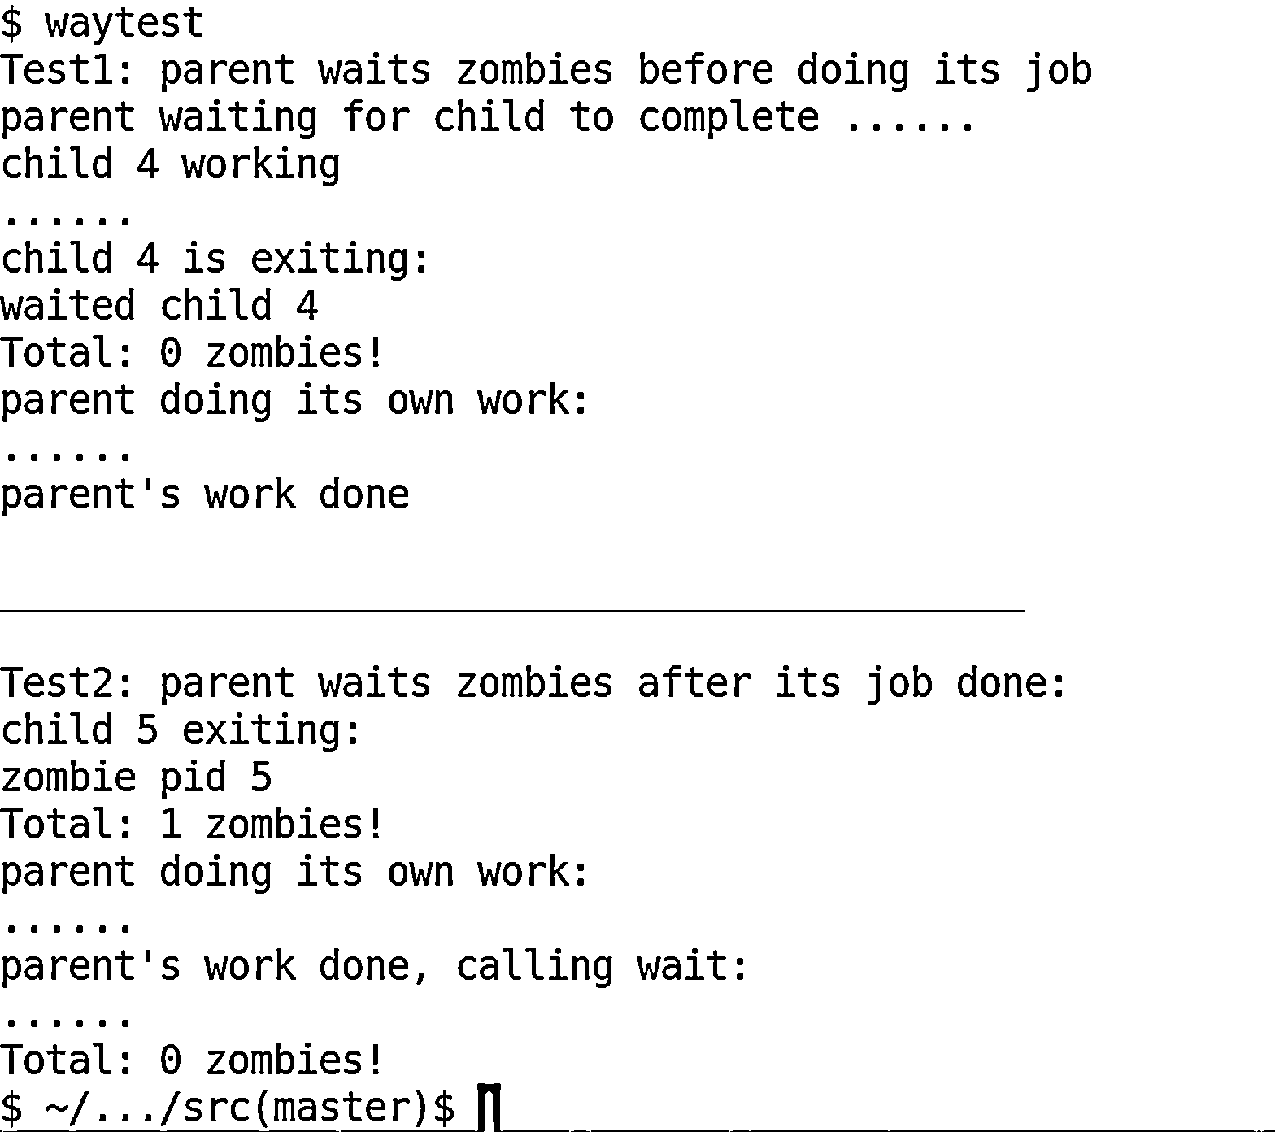
\includegraphics[width=.7\textwidth]{waytest}
  \bicaption{\texttt{waytest.c}的输出结果}{The output of \texttt{waytest.c}}
  \label{fig:waytest}
\end{figure}

\texttt{waytest1.c}运行于本文重新设计后的系统内,其运行结果输出图则如图\ref{fig:waytest1}所
示。由于经过重新设计,所有的僵尸进程的处理工作都交给了调度器来完成,也就是说任何的母进程都
不再需要担负起为子进程处理僵尸进程的任务,所以,在\texttt{waytest1.c}程序中,母进程自始至终
都不需要调用\texttt{wait()}进行僵尸进程处理,而是在创建完成子进程(
图\ref{fig:waytest1}中的\texttt{child pid 4})后便直接开始自身的工作。虽然在运行的过程中,
子进程先于母进程而退出了,但是母进程并不需要停下手中的工作来为其进行僵尸进程处理而是继续执
行自身的工作。最后当母进程执行完毕后,通过\texttt{lszombies()}工具查看先前已退出的子进程的
僵尸进程是否还存在,而此时\texttt{lszombies()}的返回结果是:系统里的僵尸进程总数为零,也就
是说僵尸进程已经被别的进程(调度器)处理了,这就表明了经过本文的重新设计后,僵尸进程的处理
工作不再需要依赖于母进程。

\begin{figure}
  \centering
  \includegraphics[width=.8\textwidth]{waytest1}
  \bicaption{\texttt{waytest1.c}的输出结果}{The output of waytest1.c}
  \label{fig:waytest1}
\end{figure}

对比\texttt{waytest.c}与\texttt{waytest1.c}的输出结果,可以看出本文所实现的处理方式的优点
是:不需要母进程的任何等待操作即可完成僵尸进程的处理工作,这就从根本上解决了母进程因等待子进程的
退出而造成自身任务被推迟的问题。

\section{资源回收的速度对比}

为了提高系统对资源的回收利用率,系统需要及时对每一个已经运行结束的进程进行资源回收。系统处
理进程退出的过程实际上就是系统对僵尸进程资源回收的一个过程。由于Linux系统把僵尸进程的处理
工作交给了母进程来处理,导致了系统对僵尸进程所占资源的回收利用存在着时间延迟。本文通过把僵
尸进程的处理工作交给调度器来完成以达成对僵尸进程所占资源的快速回收,以此提高系统的资源的回
收利用率。接下来,本文将通过实验测试来证明,本文所实现的方法确实能够大大提高回收僵尸进程所占资源
的速度。测试的所需完成的主要工作包括:
\begin{enumerate}
\item 实现一个系统调用\texttt{getfreepages()},用于随时查看系统内物理内存空闲页面总数,以
  及两个小程序:\texttt{ztime.c}和\texttt{ztime1.c},用于测试资源回收的速度。其中\texttt{ztime.c}运
  行于未经本文改变前的Linux系统,而\texttt{ztime1.c}则运行于经本文重新设计后的系统。
\item 对实验结果进行对比分析,以突出本文所实现方法能够在很大程度上提高资源的回收利用率的这
  一优点。
\end{enumerate}

\subsection{工具实现}

在未经改变前的Linux系统中,当一个进程调用\texttt{exit()}函数进行退出后,进程只是释放了CPU资源,而本身
 所占用的内存资源却尚未被释放。接下来,进程则以僵尸进程的身份继续存在系统中,以等待被母进程处理。母进程
 则通过调用\texttt{wait()}函数来释放僵尸进程的资源,所以当\texttt{wait()}函数返回的时候就表明
 僵尸进程的内存资源已经被释放回收了。为了验证僵尸进程的内存资源是否已经被释放了,本文实现
 了一个工具:\texttt{getfreepages()}系统调用,用于输出系统内当前时刻物理内存的空闲页面总数。用户可通过这
 个系统调用对比在调用\texttt{wait()}函数前与调用\texttt{wait()}函数后,内存空闲页面的总数的变化情
 况来判断内存是否得到了释放回收。负责处理\texttt{getfreepages()}系统调用的内核函数
 \texttt{getfreepages()}的具体实现如图\ref{fig:lst:freepagescode}所示。

 \begin{figure}[H]
  \begin{codeblock}
\begin{ccode}
uint getfreepages(void)
{
  uint numfreepgs;
  acquire(&kmem.lock);
  numfreepgs=kmem.freepages;
  release(&kmem.lock);
  return numfreepgs;
}
\end{ccode}
  \end{codeblock}
  \bicaption{\texttt{getfreepages()}函数的代码}{The implementation of \texttt{getfreepages()}}\label{fig:lst:freepagescode}
\end{figure}

\texttt{ztime.c}与\texttt{ztime1.c}程序的主要作用是测试系统回收僵尸进程资源的速度,其中
\texttt{ztime.c}运行于未经本文改变前的Linux系统,而\texttt{ztime1.c}则运行于经本文重新设计
后的Linux系统。由于僵尸进程被清除完成的时刻即是资源回收完成的时刻,所以,回收僵尸进程资源的
速度直接与系统清除僵尸进程的快慢程度相关。在未经本文改变前,Linux通过母进程的等待操作来
清除僵尸进程,而经过本文的重新设计后,则是通过调度器来完成清除工作。两者的区别是:前者完成
僵尸进程的清除工作需要花费的时间是子进程调用\texttt{exit()}结束后与母进程调用
\texttt{wait()}返回后的这两个时间点的差值,而后者需要花费的时间则是子进程调用
\texttt{exit()}结束后与\texttt{cleanup()}函数返回后的这两个时间点的差值。在测试的时候,为了获得这两个差
值,本文在\texttt{exit()}、\texttt{wait()}和\texttt{cleanup()}这几个函数返 
回前输出系统当前的时刻值(以时钟\texttt{ticks}值表示),再通过这些返回值来计算出时间差值。

\texttt{ztime.c}与\texttt{ztime1.c}程序首先通过调用\texttt{getfreepages()}系统调用来观察母进程在创建子进程前
后的物理内存空闲页面的总数变化来获知子进程总共占用的内存页面数目;然后在子进程调用完成
\texttt{exit()}函数后再次观察内存空闲页面总数是否有所变化;最后在\texttt{ztime.c}中的母进
程调用\texttt{wait()}函数后再次查看内存空闲页面总数的变化情况。由于经过本文重新设计后,僵
尸进程资源的回收处理不需要通过\texttt{wait()}来完成,所以,这一步在\texttt{ztime1.c}中可以
省略。\texttt{ztime.c}与\texttt{ztime1.c}的程序代码参见附录\ref{sec:spdcmp}。


\subsection{实验结果分析对比}

程序\texttt{ztime.c}和\texttt{ztime1.c}的输出结果分别如
图\ref{fig:ztime-log}和图\ref{fig:ztime1-log}所示。这两个输出结果都分为两部分:第一部分是在
子进程退出时,就绪队列里只存在一个进程即母进程的情况下测试系统回收僵尸进程资源所需的时间的
输出结果;第二种情况则是在就绪队列里有多个进程的情况下的测试输出结果。从
图\ref{fig:ztime-log}的\texttt{Test1}输出结果中,可以看出创建一个子进程(\texttt{pid 4})需
要花费$56727-56659=68$个空闲页面。接下来,子进程在第431个\texttt{tick}的时候退出了,此时系
统内的空闲页面总数仍然是56659,并没有因为子进程的退出而增加。而当僵尸进程\texttt{pid
  4}在第432个\texttt{tick}的时刻被清除后,系统内空闲页面总数增加到了创建子进程前的总数
(56727),这就表明了,只有在僵尸进程被清理完成后,系统才能回收进程所占用的资源。并且,在就
绪队列里只有一个进程的情况下,僵尸进程从产生到被完全处理的这个过程,经历
了$432-431=1$个
\texttt{tick}。一个\texttt{tick}的值相当于10ms,如果以$Z_t$表示这个过程需要花费的时间的话,
那么$Z_t=1×10ms=10ms$。而从\texttt{Test2}的输出结果可以看出,当就绪队列里的进程数量增加
时,$Z_t$的值也随之增加。接下来,将以\texttt{np}表示进程的数量,从输出结果可以看出:
\begin{itemize}
\item 当\texttt{np}的值为10的时候,$Z_t$的值就增加
  到$854-844=10$个\texttt{ticks},即$100ms$。
\item 当\texttt{np}的值为20的时候,$Z_t$的值就增加到20个\texttt{ticks},即$200ms$。
\item 当\texttt{np}的值为30的时候,$Z_t$的值就增加到30个\texttt{ticks},即\texttt{300ms}。
\item ......
\item 当\texttt{np}的值为100的时候,$Z_t$的值就增加
  到100个\texttt{ticks},即\texttt{1000ms}。
\end{itemize}

这就表明:在没有经过本文的重新设计的情况下,系统回收一个僵尸进程的时间与系统内的进程
数量有直接关系:进程数量越多,系统回收僵尸进程资源所需要的时间就越长,即速度越慢。回
收僵尸进程资源所需的时间与就绪队列里进程的数量之间的关系可用$Z_t=K*T_0$ 表示,其中\texttt{K}代表就绪队列中的进程数量,$T_0$则代表在就绪队列里只有母进程唯一一个进
程的理想情况下回收僵尸进程所需要的时间。从实验结果图\ref{fig:ztime-log}可得出,当$K=1$时,
$Z_t=T_0=10ms$。 

从\texttt{ztime1.c}的输出结果(图\ref{fig:ztime1-log})可以看出,母进程创建一个子进程同样消
耗了$56729-56661=68$个内存页面。不一样的地方是,在只有一个母进程的情况下,子进程退出成为僵
尸进程的时刻是第263个\texttt{tick},而这个僵尸进程被处理的时刻也是在第263个\texttt{tick},
这就表明了在经过本文的重新设计后,僵尸进程从产生到被清除只经历了0($263-263=0$)个tick,即
僵尸进程的处理时间降到了10ms以下。如果将这个时间精确到微秒(microsecond)级别后则是
2395($9383-6988=2395$)μs。在僵尸进程被清除后,系统内的空闲页面总数增加到了创建
子进程前的总数(56729),这就表明了随着僵尸进程被清除的同时,系统也完成了对进程资源的回收。
最后,从这个输出结果(图\ref{fig:ztime1-log})可以得出,经过重新设计后系统回收僵尸进程所需的时
间($Z_t$)与进程数量(np)之间的对应关系如下所示:
\begin{itemize}
\item 当np的值为1的时候,$Z_t$的值是2395($9383-6988=2395$)μs。
\item 当np的值为10的时候,$Z_t$的值则是660($1770-510=1260$)μs。
\item 当np的值为20的时候,$Z_t$的值则是2456($3693-1237=2456$)μs。
\item 当np的值为30的时候,$Z_t$的值则是2417($3152-735=2417$)μs。
\item ......
\item 当np的值为100的时候,$Z_t$的值则是2602($3092-490=2602$)μs。
\end{itemize}
如果以毫秒(millisecond)的形式表示$Z_t$的值的话,则np与$Z_t$之间的对应关系如下:
\begin{center}{\footnotesize
  \begin{tabular}{rccccccccccc}
    $\mathbf{np:}$&1&10&20&30&40&50&60&70&80&90&100\\[-3ex]
    $\mathbf{Z_t}:$&2.395& 1.260& 2.456& 2.417&  2.315& 2.381& 2.453& 2.544& 2.924& 2.505& 2.602
  \end{tabular}}
\end{center}
% 从\texttt{Test1}与\texttt{Test2}的输出结果来
% 看,经过本文的重新设计后,系统回收僵尸进程资源的所需要的时间与进程数量无关:无论就绪队列内是有一个进
% 程还是多个进程,系统回收僵尸进程资源的时间耗费$Z_t$都小于10ms,即小于原来的Linux系统所需的
% 时间耗费。

% 与\texttt{ztime.c}的输出
% 结果(图\ref{fig:ztime-log})对比,足以看出本文所实现的方法大大提高了系统回收僵尸进程资源的速度。

\begin{figure}
  \centering
  \fbox{\includegraphics[height=.95\textheight]{ztime-log}}
  \bicaption{\texttt{ztime.c}的输出结果}{The output of \texttt{ztime.c}}
  \label{fig:ztime-log}
\end{figure}

\begin{figure}
  \centering
  \fbox{\includegraphics[height=.95\textheight]{Ztime}}
  \bicaption{\texttt{ztime1.c}的输出结果}{The output of \texttt{ztime1.c}}
  \label{fig:ztime1-log}    
\end{figure}

对比\texttt{ztime.c}的输出结果图\ref{fig:ztime-log}和\texttt{ztime1.c}的输出结果
图\ref{fig:ztime1-log},可知:在原来的linux系统中,回收僵尸进程资源所需要的时间
可由公式$Z_t=K*T_0$ 表示,其中\texttt{K}代表就绪队列中的进程数量,$T_0$则代表在就绪队列里只有母进程唯一一个进
程的理想情况下回收僵尸进程所需要的时间,也就是10ms。
然而,在经过本文的重新设计后,系统回收
僵尸进程所需的时间与就绪队列里进程的数量无关,无论就绪队列里是有1个进程还是100个进程,
$Z_t'$的值都处于$1.260ms~2.924ms$之间,都小于10ms。因此,可得出结论:经过本文的重新
设计后,在很大程度上提高了系统回收僵尸进程资源的速度。最后,本文将原来的Linux系统回收僵尸
进程所需的时间$Z_t$与经本文重新设计后的
系统回收僵尸进程上所需的时间$Z_t'$的对比情况做成图表,如图\ref{fig:timecmp}所示。    

\begin{figure}
  \centering
  \includegraphics[width=.8\textwidth]{timecmp}
  \bicaption{回收僵尸进程资源所需的时间对比图}{The comparison of resources releasing time
    of zombie collection}
  \label{fig:timecmp}
\end{figure}

\section{安全性对比}

Linux系统把处理每个僵尸进程的工作都交给了进程各自的母进程来完成。这种依赖于母进程的等待操
作来完成资源回收的方式存在着安全隐患,毕竟用户进程不一定是安全可靠。如果一个用户编程不当,
可能造成系统内长时间存在着若干个僵尸进程,这种情况虽然不会造成什么严重的后果。但是如果遇上一个
恶意用户进程,情况就没有这么乐观了。如果一个母进程在短时间内创建了大量的子进程后,便开始了
自己的无限循环“工作”,而那些子进程实际上并没有做任何事情就直接退出了,但是由于母进程故意
“迟迟”不对任何的僵尸进程进行清除而导致掌握在这大批量的僵尸进程手中的资源一直得不到回收释放,
而最终导致系统资源的耗尽。本文为了解决这种安全隐患,改变了依赖于母进程的等待操作来进行僵尸
进程资源回收的方式,而是利用调度器来代替母进程完成资源回收。这么做的好处是:调度器是系统进
程,安全可靠,最主要是它必然会在
每一次发生进程退出时自动介入运行,所以,只要进程一旦退出成为僵尸进程后,立马就会被调度器自
动进行资源回收。接下来,为了验证本文所实现的方法确实解决了Linux处理僵尸进程流程中存在的安
全问题,本文编写了一个小程序,\texttt{Zattack.c},用于模拟恶意用户进程的攻击。

\subsection{工具实现}
进程表是Linux系统里用于存放所有进程控制块的一个数据结构,内核每创建一个进程,都需要从这个
数据结构里申请一个空位置(slot),用来存放该进程的各种状态信息。所以,如果进程表满了的话,内核便因
无法申请到一个空的\texttt{slot}来存放新进程的信息而导致创建新进程的操作失败,而无法创建新进程就意
味着无法执行新任务。为了方便实验,本文将进程表的最大容量值\texttt{MAXPROC}设置为100。在
\texttt{Zattack.c}中,程序首先创建了一个进程用于运行\texttt{Zattack()}函数,该函数的核心工作是模拟
一个恶意进程通过短期内产生大量的僵尸进程来试图耗光进程表的资源。\texttt{Zattack}进程试图创
建100个子进程,这些子进程在创建后并没有执行任何任务而是直接退出成为了僵尸进程。而
\texttt{Zattack}进程本身作为母进程却没有调用\texttt{wait()}函数对任何的僵尸进程进行资源回收,而
是开始自身的“毫无意义”的无限循环。在\texttt{Zattack}进程启动后,\texttt{Zattack.c}程序尝试创建新的进程以执行
新的任务,以验证系统是否受到恶意进程\texttt{Zattack}的影响。为了提高测试的准确性,程序每隔
两秒钟进行一次继续创建新进程的尝试,并且总共尝试十次。\texttt{Zattack.c}程序将先后运行于未
经本文改变前的Linux系统内以及经本文重新设计后的Linux系统内,以通过输出结果的区别来验证本文
所实现方法能成功提高系统的安全性,\texttt{Zattack.c}具体实现参见附录\ref{sec:seccmp}。%{fig:lst:Zattack.c}

\subsection{输出结果分析对比}
将\texttt{Zattack.c}程序运行于未经本文改变前的Linux系统内得到的输出结果如
图\ref{fig:Zattack}所示。

\begin{figure}[bh]
  \centering
  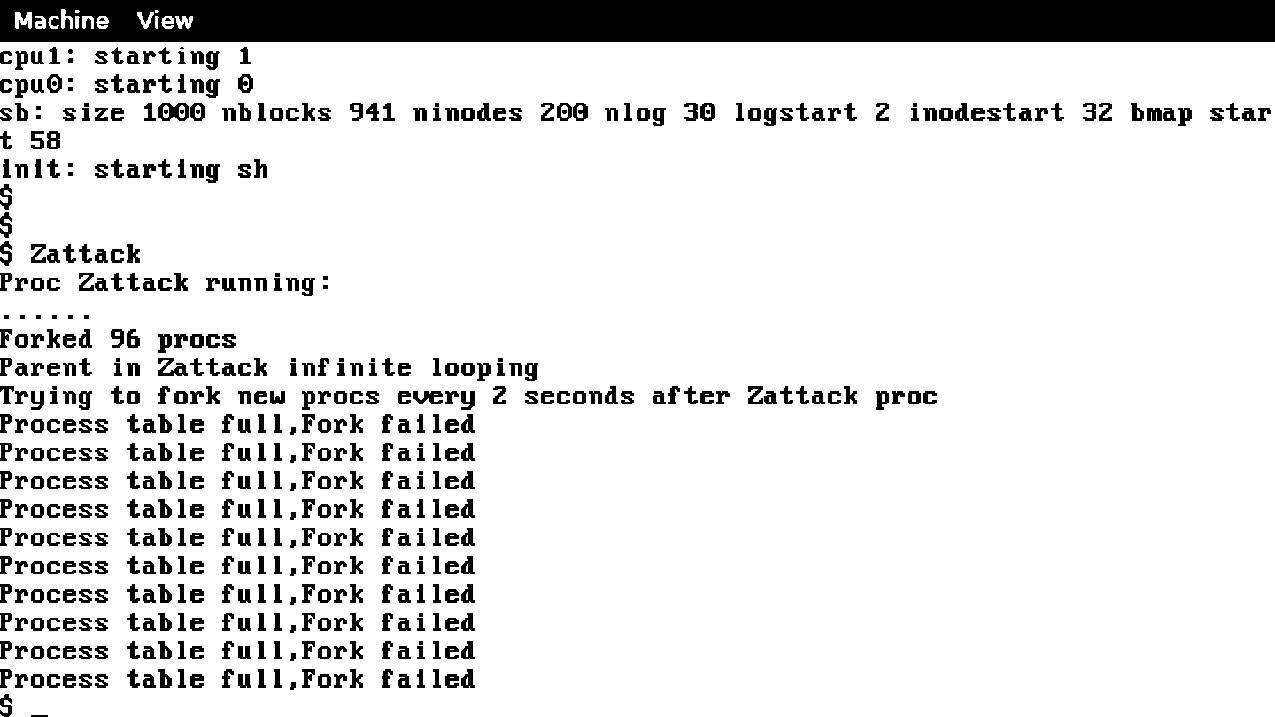
\includegraphics[width=\textwidth]{Zattack}
  \bicaption{\texttt{Zattack.c}在未经改变前的系统内运行的输出结果}{The system output
    before modifying \texttt{Zattack.c}}
  \label{fig:Zattack}
\end{figure}

\begin{figure}
  \centering
  \includegraphics[width=\textwidth]{Zattack1}
  \bicaption{\texttt{Zattack.c}在重新设计后的系统内运行的输出结果}{The system output after
  redesigning \texttt{Zattack.c}}
  \label{fig:Zattack1}    
\end{figure}

而运行于经过本文重新设计后的Linux系统内得出的输出结果则如
图\ref{fig:Zattack1}所示。
从图\ref{fig:Zattack}可以看出,虽然\texttt{Zattack}进程试图创
建100个子进程,但是最终在创建完第96个子进程后便无法再继续创建子进程了,原因是进程表的最多只
能容纳100个进程,而这其中包括了\texttt{init}进程、\texttt{shell}进程、运
行\texttt{Zattack.c}的进程以及运行\texttt{Zattack()}函数的进程,而除去这四个进程所占的位置
后,进程表里就只剩下96($100-4=96$)个空位置了。在创建完96个子进程后,进
程\texttt{Zattack}便开始进入了无限循环,此后,系统了开始以每隔两秒终创建一个新进程的尝试,
并且总共尝试了10次,但最后都是以失败告终。原因就是\texttt{Zattack}进程创建的僵尸进程一直没
有得到清除而导致进程表一直处于“被占满”状态从而导致了所有创建新进程的操作都失败。这种情况带
来的严重后果就是:系统形同瘫痪,无法再执行任何的新任务。

从图\ref{fig:Zattack1}可以看出:一开始的\texttt{Zattack}进程试图创建100个子进程
的时候,却没有因为进程表里只有96个空位置而受限,原因就是,每一个被\texttt{Zattack}进程创建
的子进程在被创建完成后立马就退出了,而经过本文的重新设计后,进程退出后几乎是立马就被资源回
收了(这一点在上一节已经被实验验证过了)。同样情况,虽然\texttt{Zattack}进程试图通过创建
100个僵尸进程来绝对占满整个进程表的空间,以阻止系统继续创建新进程,但是事实却是:系统在
\texttt{Zattack}进程启动后,做了10次尝试创建新进程的举动,而每一次尝试的结果都是成功的。这
就表明了,经过重新设计与实现后,系统具备了避免\texttt{Zattack}进程攻击的能力。这也验证了本
文所实现方法的优点:可成功避免原Linux系统处理僵尸进程的过程中存在的安全隐患,因此大大提高
了系统的安全性。

至此,本文通过三个测试验证了本文所实现的方法与原Linux的处理方法相比,具有
三个优点:
\begin{enumerate}
\item 无需依赖于母进程等待即可实现对僵尸进程的处理;
\item 能够更快速回收僵尸进程的资源;
\item 能够避免原Linux处理流程中存在的安全隐患,安全性更高。
\end{enumerate}


% \section{进程切换的时间对比}
% 在前三个小节里,本文通过三个测试验证了本文所实现的方法与原Linux的处理方法相比,具有
% 三个优点:无需依赖于母进程等待、能更快速回收僵尸进程资源、安全性更高。
% 然而,由于本文所实现的方法涉及到了调度器进程的更改,而调度器进程负责系统里的每一次进
% 程切换,因此进程切换的时间不应该太长,而且应该越短越好。本文在对Linux处理进程退出的过程进
% 行重新设计的时候也考虑这个问题,在采取把回收僵尸进程资源交给调度器实现的同时努力做到尽量不
% 增加系统进行进程切换的时间。所以,接下来,为了进一步说明本文所现方法的
% 效率性,本文将通过测试验证:
% 本文所实现的方法在具备以上所说的三个优点的同时,并没有显著增加调度器进程的工作强度,即不
% 会显著增加系统进行进程切换的时间。




\chapter{总结与展望}
僵尸进程是Linux系统处理进程退出事务的过程中产生的一种处于特殊状态的进程,僵尸进程虽然不再运行,但是
仍然占用着各种内存资源。僵尸进程产生后便一直处于系统中,直到被系统清除处理后才会消失。为了提高
系统系统对内存资源的回收利用率,必须尽早处理僵尸进程。
本文关注的是Linux处理进程退出过程中对僵尸进程资源的回收问题,针对Linux处理过程中存在的必须依赖于母进程进程的
等待来回收僵尸进程的资源而造成的资源回收速度不够的快的问题以及存在安全隐患的问题,本文提出
了采用调度器来替代母进程进行僵尸进程资源回收的新方法。总的来说,本文是从以下几个方面来完成论文的研究:
\begin{enumerate}
\item 提取Linux系统处理进程退出事务的过程模型,从本质上分析了僵尸进程产生的根源以及Linux
  对此的处理过程,并指出了Linux处理流程中潜在的必须依赖于母进程的等待操作、回收僵尸进程资
  源速度过慢、以及存在安全隐患的三个问题。
\item 面对Linux处理流程中存在的三个问题,本文提出了一种能够无需依赖于母进程的等待操作即可
  快速、安全可靠地回收僵尸进程资源的新方法,即采用调度器来替代母进程进行僵尸进程资源回收的方法。本文对所
  提的方法进行了方案设计,首先从局部开始,一一解决Linux流程中存在的这三个问题,然后在基于局部设计的基础上,
  进行通盘考虑,最终设计出一个能够同时解决这三个问题的全局解决方案,即通过采用\texttt{exit()}
  函数负责大部分的进程资源回收工作而调度器只负责少部分无法由\texttt{exit()}完成的回收工作
  的共同合作的方式来完美地达到同时解决这三个问题的目标。
\item 本文对所设计的方案进行了详细的编程实现,并通过实验分别从三个方面测试验证了本文所实现
  的方法与Linux原来的处理方法相比具有无需依赖于母进程、能够更快速地回收僵尸进程资源、能够
  避免安全隐患这三个优点,即本文成功做到了能够同时解决Linux处理流程中存在的三个问题。
\end{enumerate}

在将来的学习和工作中,本人将从以下两个方面展开后续的研究:
\begin{itemize}
  \item 目前本文只是在虚拟机(QEMU)里进行测试验证了本文所实现的方法的正确性与有效性,但是尚
  未完成把经过本文重新设计后的内核用于实际机器上运行测试这一步,因此,暂时无法预测本文所实现的方法是
  否会对系统运行的稳定性产生影响。
\item 本文在重新设计回收僵尸进程的过程中,做到了无需依赖于母进程的等待操作这一点,但是却尚
  未考虑到取消母进程的等待操作是否会影响母进程对子进程的运行信息的收集这一点。今后,本人将
  通过不懈努力,做到这一点。 
\end{itemize}


\appendix
\makebib

% 附录章节从这里开始

\chapter{主要代码清单}
\singlespacing

\section{处理方式对比}
\label{sec:cmp}

\subsection{\texttt{waytest.c}}
\label{sec:textttwaytest.c}

\begin{ccode}
#include "types.h"
#include "stat.h"
#include "user.h"

void waytest1()
{
    int pid,pid1;
    pid=fork();
    if(pid==0)
        {
            printf(1,"child %d working\n......\n",getpid());
            sleep(200);
            printf(1,"child %d is exiting:\n",getpid());
            exit();
        }
    printf(1,"parent waiting for child to complete ......\n");
    pid1=wait();
    if(pid1>0)
        {
            printf(1,"waited child %d\n",pid1);
        }
    lszombies();
    printf(1,"parent doing its own work:\n......\n");
    sleep(300);
    printf(1,"parent's work done\n");
    
}

void waytest2()
{
    int pid;
    pid=fork();
    if(pid==0)
    {
      printf(1,"child %d exiting:\n",getpid());
      exit();
    }
    lszombies();
    printf(1,"parent doing its own work:\n......\n");
    sleep(300);
    printf(1,"parent's work done, calling wait:\n......\n");
    wait();
    lszombies();
}

int main(void)
{
  printf(1,"Test1: parent waits zombies before doing its job\n");
  waytest1();
  printf(1,"\n_____________________________________________\n\n");
  printf(1,"Test2: parent waits zombies after its job done:\n");
  waytest2();
  exit();
}
\end{ccode}

\subsection{\texttt{waytest1.c}}
\label{sec:textttwaytest1.c}

\begin{ccode}
#include "types.h"
#include "stat.h"
#include "user.h"

int main(void)
{
  int pid;
  pid=fork();
  if(pid==0)
  {
    printf(1,"child %d is working\n......\n",getpid());
    sleep(200);
    printf(1,"child %d exiting!\n",getpid());
    exit();
  }
  printf(1,"parent doing its own work\n......\n");
  sleep(300);
  printf(1,"parent's work is done\n");
  lszombies();
  exit();
}
\end{ccode}

\clearpage
\section{资源回收速度对比}
\label{sec:spdcmp}

\subsection{\texttt{ztime.c}}
\label{sec:textttztime.c}

\begin{ccode}
#include "types.h"
#include "stat.h"
#include "user.h"

int test1(void)
{
    int pid;
    printf(1,"%d freepages in system before forked \n",getfreepages());
    pid=fork();
    if(pid==0)
        {
            printf(1,"%d freepages in system after forked\n",getfreepages());
            exit();
        }
    sleep(2);   
    printf(1,"%d freepages in system after exited\n",getfreepages());
    wait();
    printf(1,"%d freepages in system after waited\n",getfreepages());
    return 1;
}

int test2(void)
{
    int pid,i,pid1;
    
    pid=fork();
    if(pid==0)
        {
            sleep(200);
            exit();
        }
    for(i=1;i<=10;i++)
        {
            pid1=fork();
            if(pid1==0){
                while(1);}
        }
    wait();
    return 1;
}

int main(void)
{
    int i;
    printf(1,"\nTest1: With only 1 proc in ready queue when child exited\n");
    test1();
    for(i=1;i<=10;i++){
        printf(1,"\nTest2: With %d procs in ready queue when child exited\n",i*10);
    test2();}
    exit();
}
\end{ccode}

\subsection{\texttt{ztime1.c}}
\label{sec:ztime1.c}

\begin{ccode}
#include "types.h"
#include "stat.h"
#include "user.h"

int test1(void)
{
    int pid;
    printf(1,"%d freepages in system before forked \n",getfreepages());
    pid=fork();
    if(pid==0)
        {
            printf(1,"%d freepages in system after forked\n",getfreepages());
            exit();
        }
    sleep(2);   
    printf(1,"%d freepages in system after exited\n",getfreepages());
  return 1;
}

int test2(void)
{
    int pid,i,pid1;
    pid=fork();
    if(pid==0)
  {
    sleep(200);
    exit();
  }
    for(i=1;i<=10;i++)
        {
            pid1=fork();
            if(pid1==0){
                while(1);}
        }
  sleep(300);
  return 1;
}

int main(void)
{
  int i;
    printf(1,"\nTest1: With only 1 proc in ready queue when child exited\n");
    test1();
  for(i=1;i<=10;i++){
    printf(1,"\nTest2: With %d procs in ready queue when child exited\n",i*10);
    test2();
  }
  exit();
}
\end{ccode}

\section{安全性对比}
\label{sec:seccmp}

\texttt{Zattack.c}程序的代码:

\begin{ccode}
#include"types.h"
#include"stat.h"
#include"user.h"

int Zattack(void)
{
    int pid1,i;
    for(i=1;i<=100;i++)
        {
            pid1=fork();
            if(pid1<0)
                {   printf(1,"Forked %d procs\n",i);
                    break;
                }
            if(pid1==0)
                {
                    exit();
                }
        }
    if(i>=100)
        printf(1,"Fork claimes to work 100 times\n");
    printf(1,"Parent in Zattack infinite looping\n");
    while(1);
    return 1;
}

int main(void)
{
    int pid,pid1,i;
    pid1=fork();
    if(pid1==0)
        {
            printf(1,"Proc Zattack running:\n......\n");
            Zattack();
        }
    sleep(500);
    printf(1,"Trying to fork new procs every 2 seconds after Zattack proc\n");
    for(i=1;i<=10;i++)
        {
            pid=fork();
            if(pid<0)
                {
                    printf(1,"Process table full,Fork failed\n");
                }
            else if(pid==0)
                exit();
            else
                printf(1,"Forked new proc %d\n",pid);
            sleep(200);
        }
    exit();
}
\end{ccode}

%%% tail pages
\doublespacing

\begin{authorInfo}
  罗志兵(1989 ─),女,广西贵港人,本科毕业于西南林业大学
  计算机与信息科学学院,现为在读硕士研究生,就读于西南林业大学大数据与智能工程学院,所学专
  业为林业信息工程。曾发表的论文有《基于动态规划的基因双序列比对研究》。
\end{authorInfo}

\begin{advisorInfo}
  赵家刚,硕士研究生、副教授,硕士研究生导师,云南省科技项目评审专家,云南省计算机协会理事,
  主要研究智能数据处理、信息系统开发。主持了多个项目,主编教材3部。

  主讲的课程有《C语言程序设计》、《面向对象程序设计》、《数据结构》、《图形图像程序设计》、
  《人工智能》、《人工神经网络》、《组件技术》、《离散数学》、《计算机编程导论》。

  \noindent{}•\, 主要学习、工作经历:
  \begin{itemize}
  \item[] 1978.9-1980.7,在腾冲师范读书;
  \item[] 1980.8-1983.8,在腾冲固东中学任教;
  \item[] 1983.9-1987.7,在云南师大数学系读本科,获理学士学位;
  \item[] 1987.6-1998.8,在保山师专任计算机教学工作;
  \item[] 1998.9-2001.6,在云南师大计科系读研究生,获理学硕士学位;
  \item[] 2001.7-至今,在西南林学院计科系工作。主要从事软件开发的教学工作,培养了众多编程高
    手。
  \end{itemize}

  \noindent{}•\, 主要论著和文章:
  \begin{refsection}
    \nocite{zjg02,zjg03,zjg07,zjg09,zjg09-2,zjg09-3,zjg09-4,zjg10,zjg11,zjg13}
    \printbibliography[heading=none] 
  \end{refsection}

  \noindent{}•\, 主持的项目:
  \begin{enumerate}
  \item 2003.6-2004.5,西南林学院,``数据结构教学改革研究'';
  \item 2007.5-2008.12,云南海诚集团,``项目建设工程数据库管理软件'',具有工作流;
  \item 2008.6-2009.6,昆明市科计局科技项目审批软件,具有工作流;
  \item 2010.10-2013.10,科学出版社大型教育类网站研发;
  \item 2013.10-2016.10,云南省委组织部办公邮件系统。
  \end{enumerate}
\end{advisorInfo}

\publication{luo17}

\begin{acknowledgment}
  本课题和论文的完成得到了许多老师和同学的支持和帮助,在这里,我将给予他们最衷心的感谢。在
  这里,感谢我的导师,赵家刚以及代飞老师的悉心指导和帮助,使得该论文能如期完成。从选择研究
  方向到确定具体的实施方案,从论文的初稿到最后的审定,无不花费了他大量的心血和精力。 赵老师
  和代老师的博学多才,和他们在科研学术方面的认真、严谨、求实、创新的态度, 以及开拓进取的工
  作作风都让我收益匪浅。
\end{acknowledgment}

\end{document}



%%% Local Variables:
%%% mode: latex
%%% TeX-master: t
%%% End:
